% Options for packages loaded elsewhere
\PassOptionsToPackage{unicode}{hyperref}
\PassOptionsToPackage{hyphens}{url}
%
\documentclass[
]{article}
\usepackage{amsmath,amssymb}
\usepackage{lmodern}
\usepackage{iftex}
\ifPDFTeX
  \usepackage[T1]{fontenc}
  \usepackage[utf8]{inputenc}
  \usepackage{textcomp} % provide euro and other symbols
\else % if luatex or xetex
  \usepackage{unicode-math}
  \defaultfontfeatures{Scale=MatchLowercase}
  \defaultfontfeatures[\rmfamily]{Ligatures=TeX,Scale=1}
\fi
% Use upquote if available, for straight quotes in verbatim environments
\IfFileExists{upquote.sty}{\usepackage{upquote}}{}
\IfFileExists{microtype.sty}{% use microtype if available
  \usepackage[]{microtype}
  \UseMicrotypeSet[protrusion]{basicmath} % disable protrusion for tt fonts
}{}
\makeatletter
\@ifundefined{KOMAClassName}{% if non-KOMA class
  \IfFileExists{parskip.sty}{%
    \usepackage{parskip}
  }{% else
    \setlength{\parindent}{0pt}
    \setlength{\parskip}{6pt plus 2pt minus 1pt}}
}{% if KOMA class
  \KOMAoptions{parskip=half}}
\makeatother
\usepackage{xcolor}
\usepackage[margin=1in]{geometry}
\usepackage{color}
\usepackage{fancyvrb}
\newcommand{\VerbBar}{|}
\newcommand{\VERB}{\Verb[commandchars=\\\{\}]}
\DefineVerbatimEnvironment{Highlighting}{Verbatim}{commandchars=\\\{\}}
% Add ',fontsize=\small' for more characters per line
\usepackage{framed}
\definecolor{shadecolor}{RGB}{248,248,248}
\newenvironment{Shaded}{\begin{snugshade}}{\end{snugshade}}
\newcommand{\AlertTok}[1]{\textcolor[rgb]{0.94,0.16,0.16}{#1}}
\newcommand{\AnnotationTok}[1]{\textcolor[rgb]{0.56,0.35,0.01}{\textbf{\textit{#1}}}}
\newcommand{\AttributeTok}[1]{\textcolor[rgb]{0.77,0.63,0.00}{#1}}
\newcommand{\BaseNTok}[1]{\textcolor[rgb]{0.00,0.00,0.81}{#1}}
\newcommand{\BuiltInTok}[1]{#1}
\newcommand{\CharTok}[1]{\textcolor[rgb]{0.31,0.60,0.02}{#1}}
\newcommand{\CommentTok}[1]{\textcolor[rgb]{0.56,0.35,0.01}{\textit{#1}}}
\newcommand{\CommentVarTok}[1]{\textcolor[rgb]{0.56,0.35,0.01}{\textbf{\textit{#1}}}}
\newcommand{\ConstantTok}[1]{\textcolor[rgb]{0.00,0.00,0.00}{#1}}
\newcommand{\ControlFlowTok}[1]{\textcolor[rgb]{0.13,0.29,0.53}{\textbf{#1}}}
\newcommand{\DataTypeTok}[1]{\textcolor[rgb]{0.13,0.29,0.53}{#1}}
\newcommand{\DecValTok}[1]{\textcolor[rgb]{0.00,0.00,0.81}{#1}}
\newcommand{\DocumentationTok}[1]{\textcolor[rgb]{0.56,0.35,0.01}{\textbf{\textit{#1}}}}
\newcommand{\ErrorTok}[1]{\textcolor[rgb]{0.64,0.00,0.00}{\textbf{#1}}}
\newcommand{\ExtensionTok}[1]{#1}
\newcommand{\FloatTok}[1]{\textcolor[rgb]{0.00,0.00,0.81}{#1}}
\newcommand{\FunctionTok}[1]{\textcolor[rgb]{0.00,0.00,0.00}{#1}}
\newcommand{\ImportTok}[1]{#1}
\newcommand{\InformationTok}[1]{\textcolor[rgb]{0.56,0.35,0.01}{\textbf{\textit{#1}}}}
\newcommand{\KeywordTok}[1]{\textcolor[rgb]{0.13,0.29,0.53}{\textbf{#1}}}
\newcommand{\NormalTok}[1]{#1}
\newcommand{\OperatorTok}[1]{\textcolor[rgb]{0.81,0.36,0.00}{\textbf{#1}}}
\newcommand{\OtherTok}[1]{\textcolor[rgb]{0.56,0.35,0.01}{#1}}
\newcommand{\PreprocessorTok}[1]{\textcolor[rgb]{0.56,0.35,0.01}{\textit{#1}}}
\newcommand{\RegionMarkerTok}[1]{#1}
\newcommand{\SpecialCharTok}[1]{\textcolor[rgb]{0.00,0.00,0.00}{#1}}
\newcommand{\SpecialStringTok}[1]{\textcolor[rgb]{0.31,0.60,0.02}{#1}}
\newcommand{\StringTok}[1]{\textcolor[rgb]{0.31,0.60,0.02}{#1}}
\newcommand{\VariableTok}[1]{\textcolor[rgb]{0.00,0.00,0.00}{#1}}
\newcommand{\VerbatimStringTok}[1]{\textcolor[rgb]{0.31,0.60,0.02}{#1}}
\newcommand{\WarningTok}[1]{\textcolor[rgb]{0.56,0.35,0.01}{\textbf{\textit{#1}}}}
\usepackage{graphicx}
\makeatletter
\def\maxwidth{\ifdim\Gin@nat@width>\linewidth\linewidth\else\Gin@nat@width\fi}
\def\maxheight{\ifdim\Gin@nat@height>\textheight\textheight\else\Gin@nat@height\fi}
\makeatother
% Scale images if necessary, so that they will not overflow the page
% margins by default, and it is still possible to overwrite the defaults
% using explicit options in \includegraphics[width, height, ...]{}
\setkeys{Gin}{width=\maxwidth,height=\maxheight,keepaspectratio}
% Set default figure placement to htbp
\makeatletter
\def\fps@figure{htbp}
\makeatother
\setlength{\emergencystretch}{3em} % prevent overfull lines
\providecommand{\tightlist}{%
  \setlength{\itemsep}{0pt}\setlength{\parskip}{0pt}}
\setcounter{secnumdepth}{-\maxdimen} % remove section numbering
\ifLuaTeX
  \usepackage{selnolig}  % disable illegal ligatures
\fi
\IfFileExists{bookmark.sty}{\usepackage{bookmark}}{\usepackage{hyperref}}
\IfFileExists{xurl.sty}{\usepackage{xurl}}{} % add URL line breaks if available
\urlstyle{same} % disable monospaced font for URLs
\hypersetup{
  pdftitle={Paper 2, Econ 980x},
  pdfauthor={Alice Chen},
  hidelinks,
  pdfcreator={LaTeX via pandoc}}

\title{Paper 2, Econ 980x}
\author{Alice Chen}
\date{2022-11-27}

\begin{document}
\maketitle

\begin{Shaded}
\begin{Highlighting}[]
\NormalTok{ddi }\OtherTok{\textless{}{-}} \FunctionTok{read\_ipums\_ddi}\NormalTok{(}\StringTok{"atus\_00005.xml"}\NormalTok{)}
\NormalTok{csv }\OtherTok{\textless{}{-}} \FunctionTok{read\_ipums\_micro}\NormalTok{(ddi) }\SpecialCharTok{\%\textgreater{}\%}
  \FunctionTok{clean\_names}\NormalTok{()}
\end{Highlighting}
\end{Shaded}

\begin{verbatim}
## Use of data from IPUMS ATUS is subject to conditions including that users
## should cite the data appropriately. Use command `ipums_conditions()` for more
## details.
\end{verbatim}

\begin{Shaded}
\begin{Highlighting}[]
\NormalTok{data}
\end{Highlighting}
\end{Shaded}

\begin{verbatim}
## function (..., list = character(), package = NULL, lib.loc = NULL, 
##     verbose = getOption("verbose"), envir = .GlobalEnv, overwrite = TRUE) 
## {
##     fileExt <- function(x) {
##         db <- grepl("\\.[^.]+\\.(gz|bz2|xz)$", x)
##         ans <- sub(".*\\.", "", x)
##         ans[db] <- sub(".*\\.([^.]+\\.)(gz|bz2|xz)$", "\\1\\2", 
##             x[db])
##         ans
##     }
##     my_read_table <- function(...) {
##         lcc <- Sys.getlocale("LC_COLLATE")
##         on.exit(Sys.setlocale("LC_COLLATE", lcc))
##         Sys.setlocale("LC_COLLATE", "C")
##         read.table(...)
##     }
##     stopifnot(is.character(list))
##     names <- c(as.character(substitute(list(...))[-1L]), list)
##     if (!is.null(package)) {
##         if (!is.character(package)) 
##             stop("'package' must be a character vector or NULL")
##     }
##     paths <- find.package(package, lib.loc, verbose = verbose)
##     if (is.null(lib.loc)) 
##         paths <- c(path.package(package, TRUE), if (!length(package)) getwd(), 
##             paths)
##     paths <- unique(normalizePath(paths[file.exists(paths)]))
##     paths <- paths[dir.exists(file.path(paths, "data"))]
##     dataExts <- tools:::.make_file_exts("data")
##     if (length(names) == 0L) {
##         db <- matrix(character(), nrow = 0L, ncol = 4L)
##         for (path in paths) {
##             entries <- NULL
##             packageName <- if (file_test("-f", file.path(path, 
##                 "DESCRIPTION"))) 
##                 basename(path)
##             else "."
##             if (file_test("-f", INDEX <- file.path(path, "Meta", 
##                 "data.rds"))) {
##                 entries <- readRDS(INDEX)
##             }
##             else {
##                 dataDir <- file.path(path, "data")
##                 entries <- tools::list_files_with_type(dataDir, 
##                   "data")
##                 if (length(entries)) {
##                   entries <- unique(tools::file_path_sans_ext(basename(entries)))
##                   entries <- cbind(entries, "")
##                 }
##             }
##             if (NROW(entries)) {
##                 if (is.matrix(entries) && ncol(entries) == 2L) 
##                   db <- rbind(db, cbind(packageName, dirname(path), 
##                     entries))
##                 else warning(gettextf("data index for package %s is invalid and will be ignored", 
##                   sQuote(packageName)), domain = NA, call. = FALSE)
##             }
##         }
##         colnames(db) <- c("Package", "LibPath", "Item", "Title")
##         footer <- if (missing(package)) 
##             paste0("Use ", sQuote(paste("data(package =", ".packages(all.available = TRUE))")), 
##                 "\n", "to list the data sets in all *available* packages.")
##         else NULL
##         y <- list(title = "Data sets", header = NULL, results = db, 
##             footer = footer)
##         class(y) <- "packageIQR"
##         return(y)
##     }
##     paths <- file.path(paths, "data")
##     for (name in names) {
##         found <- FALSE
##         for (p in paths) {
##             tmp_env <- if (overwrite) 
##                 envir
##             else new.env()
##             if (file_test("-f", file.path(p, "Rdata.rds"))) {
##                 rds <- readRDS(file.path(p, "Rdata.rds"))
##                 if (name %in% names(rds)) {
##                   found <- TRUE
##                   if (verbose) 
##                     message(sprintf("name=%s:\t found in Rdata.rds", 
##                       name), domain = NA)
##                   thispkg <- sub(".*/([^/]*)/data$", "\\1", p)
##                   thispkg <- sub("_.*$", "", thispkg)
##                   thispkg <- paste0("package:", thispkg)
##                   objs <- rds[[name]]
##                   lazyLoad(file.path(p, "Rdata"), envir = tmp_env, 
##                     filter = function(x) x %in% objs)
##                   break
##                 }
##                 else if (verbose) 
##                   message(sprintf("name=%s:\t NOT found in names() of Rdata.rds, i.e.,\n\t%s\n", 
##                     name, paste(names(rds), collapse = ",")), 
##                     domain = NA)
##             }
##             if (file_test("-f", file.path(p, "Rdata.zip"))) {
##                 warning("zipped data found for package ", sQuote(basename(dirname(p))), 
##                   ".\nThat is defunct, so please re-install the package.", 
##                   domain = NA)
##                 if (file_test("-f", fp <- file.path(p, "filelist"))) 
##                   files <- file.path(p, scan(fp, what = "", quiet = TRUE))
##                 else {
##                   warning(gettextf("file 'filelist' is missing for directory %s", 
##                     sQuote(p)), domain = NA)
##                   next
##                 }
##             }
##             else {
##                 files <- list.files(p, full.names = TRUE)
##             }
##             files <- files[grep(name, files, fixed = TRUE)]
##             if (length(files) > 1L) {
##                 o <- match(fileExt(files), dataExts, nomatch = 100L)
##                 paths0 <- dirname(files)
##                 paths0 <- factor(paths0, levels = unique(paths0))
##                 files <- files[order(paths0, o)]
##             }
##             if (length(files)) {
##                 for (file in files) {
##                   if (verbose) 
##                     message("name=", name, ":\t file= ...", .Platform$file.sep, 
##                       basename(file), "::\t", appendLF = FALSE, 
##                       domain = NA)
##                   ext <- fileExt(file)
##                   if (basename(file) != paste0(name, ".", ext)) 
##                     found <- FALSE
##                   else {
##                     found <- TRUE
##                     zfile <- file
##                     zipname <- file.path(dirname(file), "Rdata.zip")
##                     if (file.exists(zipname)) {
##                       Rdatadir <- tempfile("Rdata")
##                       dir.create(Rdatadir, showWarnings = FALSE)
##                       topic <- basename(file)
##                       rc <- .External(C_unzip, zipname, topic, 
##                         Rdatadir, FALSE, TRUE, FALSE, FALSE)
##                       if (rc == 0L) 
##                         zfile <- file.path(Rdatadir, topic)
##                     }
##                     if (zfile != file) 
##                       on.exit(unlink(zfile))
##                     switch(ext, R = , r = {
##                       library("utils")
##                       sys.source(zfile, chdir = TRUE, envir = tmp_env)
##                     }, RData = , rdata = , rda = load(zfile, 
##                       envir = tmp_env), TXT = , txt = , tab = , 
##                       tab.gz = , tab.bz2 = , tab.xz = , txt.gz = , 
##                       txt.bz2 = , txt.xz = assign(name, my_read_table(zfile, 
##                         header = TRUE, as.is = FALSE), envir = tmp_env), 
##                       CSV = , csv = , csv.gz = , csv.bz2 = , 
##                       csv.xz = assign(name, my_read_table(zfile, 
##                         header = TRUE, sep = ";", as.is = FALSE), 
##                         envir = tmp_env), found <- FALSE)
##                   }
##                   if (found) 
##                     break
##                 }
##                 if (verbose) 
##                   message(if (!found) 
##                     "*NOT* ", "found", domain = NA)
##             }
##             if (found) 
##                 break
##         }
##         if (!found) {
##             warning(gettextf("data set %s not found", sQuote(name)), 
##                 domain = NA)
##         }
##         else if (!overwrite) {
##             for (o in ls(envir = tmp_env, all.names = TRUE)) {
##                 if (exists(o, envir = envir, inherits = FALSE)) 
##                   warning(gettextf("an object named %s already exists and will not be overwritten", 
##                     sQuote(o)))
##                 else assign(o, get(o, envir = tmp_env, inherits = FALSE), 
##                   envir = envir)
##             }
##             rm(tmp_env)
##         }
##     }
##     invisible(names)
## }
## <bytecode: 0x10cead708>
## <environment: namespace:utils>
\end{verbatim}

\begin{Shaded}
\begin{Highlighting}[]
\CommentTok{\#csv \textless{}{-} read\_csv(file = "atus\_00001.csv.gz") \%\textgreater{}\%}
 \CommentTok{\# clean\_names()}

\CommentTok{\# race }
\NormalTok{race\_file }\OtherTok{\textless{}{-}} \FunctionTok{read\_excel}\NormalTok{(}\StringTok{"race\_980x.xlsx"}\NormalTok{)}

\NormalTok{race\_file }\OtherTok{\textless{}{-}}\NormalTok{ race\_file }\SpecialCharTok{\%\textgreater{}\%}
  \FunctionTok{rename}\NormalTok{(}\AttributeTok{code1 =}\NormalTok{ race) }\SpecialCharTok{\%\textgreater{}\%}
  \FunctionTok{rename}\NormalTok{(}\AttributeTok{race =}\NormalTok{ code) }

\NormalTok{csv }\OtherTok{\textless{}{-}} \FunctionTok{left\_join}\NormalTok{(csv, race\_file, }\AttributeTok{by =} \StringTok{"race"}\NormalTok{) }\SpecialCharTok{\%\textgreater{}\%}
  \FunctionTok{rename}\NormalTok{(}\AttributeTok{race\_code =}\NormalTok{ race) }\SpecialCharTok{\%\textgreater{}\%}
  \FunctionTok{rename}\NormalTok{(}\AttributeTok{race =}\NormalTok{ code1)}


\CommentTok{\# education}
\NormalTok{education\_file }\OtherTok{\textless{}{-}} \FunctionTok{read\_excel}\NormalTok{(}\StringTok{"Education.xlsx"}\NormalTok{)}
\NormalTok{education\_file }\OtherTok{\textless{}{-}}\NormalTok{ education\_file }\SpecialCharTok{\%\textgreater{}\%}
  \FunctionTok{rename}\NormalTok{(}\AttributeTok{code\_educ =}\NormalTok{ educ) }\SpecialCharTok{\%\textgreater{}\%}
  \FunctionTok{rename}\NormalTok{(}\AttributeTok{educ =}\NormalTok{ code\_education) }\SpecialCharTok{\%\textgreater{}\%}
  \FunctionTok{mutate}\NormalTok{(}\AttributeTok{educ =} \FunctionTok{as.numeric}\NormalTok{(educ))}

\NormalTok{csv }\OtherTok{\textless{}{-}} \FunctionTok{left\_join}\NormalTok{(csv, education\_file, }\AttributeTok{by =} \StringTok{"educ"}\NormalTok{) }\SpecialCharTok{\%\textgreater{}\%}
  \FunctionTok{rename}\NormalTok{(}\AttributeTok{code\_education =}\NormalTok{ educ) }\SpecialCharTok{\%\textgreater{}\%}
  \FunctionTok{rename}\NormalTok{(}\AttributeTok{educ =}\NormalTok{ code\_educ) }

\CommentTok{\# marital status}
\NormalTok{marital\_file }\OtherTok{\textless{}{-}} \FunctionTok{read\_excel}\NormalTok{(}\StringTok{"marital\_status.xlsx"}\NormalTok{)}
\NormalTok{education\_file }\OtherTok{\textless{}{-}}\NormalTok{ marital\_file }\SpecialCharTok{\%\textgreater{}\%}
  \FunctionTok{mutate}\NormalTok{(}\AttributeTok{marst =} \FunctionTok{as.numeric}\NormalTok{(marst))}
  
\NormalTok{csv }\OtherTok{\textless{}{-}} \FunctionTok{left\_join}\NormalTok{(csv, marital\_file, }\AttributeTok{by =} \StringTok{"marst"}\NormalTok{) }\SpecialCharTok{\%\textgreater{}\%}
  \FunctionTok{rename}\NormalTok{(}\AttributeTok{code\_marst =}\NormalTok{ marst) }\SpecialCharTok{\%\textgreater{}\%}
  \FunctionTok{rename}\NormalTok{(}\AttributeTok{marst =}\NormalTok{ marst\_code) }\SpecialCharTok{\%\textgreater{}\%}
  \FunctionTok{mutate}\NormalTok{(}\AttributeTok{marst\_simple =} \FunctionTok{ifelse}\NormalTok{(code\_marst }\SpecialCharTok{\textless{}=} \DecValTok{2}\NormalTok{, }\StringTok{"Married"}\NormalTok{, }\FunctionTok{ifelse}\NormalTok{(code\_marst }\SpecialCharTok{\textgreater{}=} \DecValTok{6}\NormalTok{, }\StringTok{"Never Married"}\NormalTok{, }\StringTok{"Separated/Divorced"}\NormalTok{)))}



\CommentTok{\# age}
\NormalTok{csv }\OtherTok{\textless{}{-}}\NormalTok{ csv }\SpecialCharTok{\%\textgreater{}\%}
  \FunctionTok{filter}\NormalTok{(age }\SpecialCharTok{\textgreater{}} \DecValTok{18}\NormalTok{)}

\CommentTok{\# children}
\NormalTok{csv }\OtherTok{\textless{}{-}}\NormalTok{ csv }\SpecialCharTok{\%\textgreater{}\%}
  \FunctionTok{mutate}\NormalTok{(}\AttributeTok{child =} \FunctionTok{ifelse}\NormalTok{(yngch }\SpecialCharTok{\textless{}} \DecValTok{19}\NormalTok{, }\DecValTok{1}\NormalTok{, }\DecValTok{0}\NormalTok{) )}

\CommentTok{\# gender}

\NormalTok{csv }\OtherTok{\textless{}{-}}\NormalTok{ csv }\SpecialCharTok{\%\textgreater{}\%}
  \FunctionTok{mutate}\NormalTok{(}\AttributeTok{gender =} \FunctionTok{ifelse}\NormalTok{(sex }\SpecialCharTok{==} \DecValTok{1}\NormalTok{, }\StringTok{"male"}\NormalTok{, }\StringTok{"female"}\NormalTok{)) }

\CommentTok{\# years }

\NormalTok{csv }\SpecialCharTok{\%\textgreater{}\%}
  \FunctionTok{summary}\NormalTok{(earnweek)}
\end{Highlighting}
\end{Shaded}

\begin{verbatim}
##       year          caseid              pernum      lineno       wt06          
##  Min.   :2003   Min.   :2.003e+13   Min.   :1   Min.   :1   Min.   :   419472  
##  1st Qu.:2006   1st Qu.:2.006e+13   1st Qu.:1   1st Qu.:1   1st Qu.:  2932235  
##  Median :2011   Median :2.011e+13   Median :1   Median :1   Median :  5230098  
##  Mean   :2011   Mean   :2.011e+13   Mean   :1   Mean   :1   Mean   :  7201674  
##  3rd Qu.:2016   3rd Qu.:2.016e+13   3rd Qu.:1   3rd Qu.:1   3rd Qu.:  8816158  
##  Max.   :2021   Max.   :2.021e+13   Max.   :1   Max.   :1   Max.   :209010030  
##                                                             NA's   :8469       
##       wt20                age             sex          race_code  
##  Min.   :        0   Min.   :19.00   Min.   :1.000   Min.   :100  
##  1st Qu.:  3606315   1st Qu.:36.00   1st Qu.:1.000   1st Qu.:100  
##  Median :  6475784   Median :48.00   Median :2.000   Median :100  
##  Mean   :  8746744   Mean   :49.48   Mean   :1.563   Mean   :104  
##  3rd Qu.: 11222184   3rd Qu.:62.00   3rd Qu.:2.000   3rd Qu.:100  
##  Max.   :137151708   Max.   :85.00   Max.   :2.000   Max.   :599  
##  NA's   :199330                                                   
##    code_marst    code_education    educyrs       empstat_cps8     fullpart    
##  Min.   :1.000   Min.   :10.0   Min.   :101.0   Min.   :1.00   Min.   : 1.00  
##  1st Qu.:1.000   1st Qu.:21.0   1st Qu.:112.0   1st Qu.:1.00   1st Qu.: 1.00  
##  Median :1.000   Median :30.0   Median :214.0   Median :1.00   Median : 1.00  
##  Mean   :2.764   Mean   :29.7   Mean   :190.4   Mean   :2.72   Mean   :37.06  
##  3rd Qu.:4.000   3rd Qu.:40.0   3rd Qu.:216.0   3rd Qu.:5.00   3rd Qu.:99.00  
##  Max.   :6.000   Max.   :43.0   Max.   :321.0   Max.   :7.00   Max.   :99.00  
##                                                                               
##     earnweek            eldch          yngch           nchild      
##  Min.   :     0.0   Min.   : 0.0   Min.   : 0.00   Min.   :0.0000  
##  1st Qu.:   673.1   1st Qu.:13.0   1st Qu.: 9.00   1st Qu.:0.0000  
##  Median :  1846.2   Median :99.0   Median :99.00   Median :0.0000  
##  Mean   : 44392.0   Mean   :60.8   Mean   :59.44   Mean   :0.8366  
##  3rd Qu.:100000.0   3rd Qu.:99.0   3rd Qu.:99.00   3rd Qu.:2.0000  
##  Max.   :100000.0   Max.   :99.0   Max.   :99.00   Max.   :9.0000  
##                                                                    
##    bls_carehh         bls_comm          bls_educ           bls_food      
##  Min.   :   0.00   Min.   :   0.00   Min.   :   0.000   Min.   :   0.00  
##  1st Qu.:   0.00   1st Qu.:   0.00   1st Qu.:   0.000   1st Qu.:  30.00  
##  Median :   0.00   Median :   0.00   Median :   0.000   Median :  60.00  
##  Mean   :  38.93   Mean   :  10.74   Mean   :   8.373   Mean   :  75.24  
##  3rd Qu.:  30.00   3rd Qu.:   0.00   3rd Qu.:   0.000   3rd Qu.: 100.00  
##  Max.   :1230.00   Max.   :1200.00   Max.   :1190.000   Max.   :1320.00  
##                                                                          
##    bls_hhact         bls_leis      bls_leis_arts      bls_leis_attend  
##  Min.   :   0.0   Min.   :   0.0   Min.   :   0.000   Min.   :  0.000  
##  1st Qu.:  15.0   1st Qu.: 155.0   1st Qu.:   0.000   1st Qu.:  0.000  
##  Median :  75.0   Median : 294.0   Median :   0.000   Median :  0.000  
##  Mean   : 124.9   Mean   : 329.4   Mean   :   5.879   Mean   :  6.128  
##  3rd Qu.: 185.0   3rd Qu.: 475.0   3rd Qu.:   0.000   3rd Qu.:  0.000  
##  Max.   :1405.0   Max.   :1439.0   Max.   :1015.000   Max.   :860.000  
##                                                                        
##  bls_leis_attsport  bls_leis_partsport bls_leis_relax    bls_leis_soc   
##  Min.   :   0.000   Min.   :   0.00    Min.   :   0.0   Min.   :   0.0  
##  1st Qu.:   0.000   1st Qu.:   0.00    1st Qu.:  90.0   1st Qu.: 130.0  
##  Median :   0.000   Median :   0.00    Median : 195.0   Median : 255.0  
##  Mean   :   1.832   Mean   :  16.25    Mean   : 245.3   Mean   : 297.7  
##  3rd Qu.:   0.000   3rd Qu.:   0.00    3rd Qu.: 356.0   3rd Qu.: 425.0  
##  Max.   :1030.000   Max.   :1125.00    Max.   :1439.0   Max.   :1439.0  
##                                                                         
##  bls_leis_soccom   bls_leis_soccomex bls_leis_sport    bls_leis_travel  
##  Min.   :   0.00   Min.   :   0.00   Min.   :   0.00   Min.   :   0.00  
##  1st Qu.:   0.00   1st Qu.:   0.00   1st Qu.:   0.00   1st Qu.:   0.00  
##  Median :   0.00   Median :   0.00   Median :   0.00   Median :   0.00  
##  Mean   :  46.38   Mean   :  40.22   Mean   :  18.15   Mean   :  13.54  
##  3rd Qu.:  60.00   3rd Qu.:  45.00   3rd Qu.:   0.00   3rd Qu.:  12.00  
##  Max.   :1350.00   Max.   :1350.00   Max.   :1125.00   Max.   :1350.00  
##                                                                         
##   bls_leis_tv       bls_pcare      bls_purch         bls_social     
##  Min.   :   0.0   Min.   :   0   Min.   :   0.00   Min.   :   0.00  
##  1st Qu.:  40.0   1st Qu.: 490   1st Qu.:   0.00   1st Qu.:   0.00  
##  Median : 122.0   Median : 564   Median :   0.00   Median :   0.00  
##  Mean   : 176.9   Mean   : 574   Mean   :  49.23   Mean   :  25.12  
##  3rd Qu.: 255.0   3rd Qu.: 645   3rd Qu.:  73.00   3rd Qu.:   0.00  
##  Max.   :1433.0   Max.   :1440   Max.   :1320.00   Max.   :1325.00  
##                                                                     
##     bls_work          race               educ              marst          
##  Min.   :   0.0   Length:216908      Length:216908      Length:216908     
##  1st Qu.:   0.0   Class :character   Class :character   Class :character  
##  Median :   0.0   Mode  :character   Mode  :character   Mode  :character  
##  Mean   : 176.7                                                           
##  3rd Qu.: 438.2                                                           
##  Max.   :1430.0                                                           
##                                                                           
##  marst_simple           child          gender         
##  Length:216908      Min.   :0.000   Length:216908     
##  Class :character   1st Qu.:0.000   Class :character  
##  Mode  :character   Median :0.000   Mode  :character  
##                     Mean   :0.385                     
##                     3rd Qu.:1.000                     
##                     Max.   :1.000                     
## 
\end{verbatim}

\begin{Shaded}
\begin{Highlighting}[]
\CommentTok{\# employed}
\NormalTok{csv }\OtherTok{\textless{}{-}}\NormalTok{ csv }\SpecialCharTok{\%\textgreater{}\%}
  \FunctionTok{mutate}\NormalTok{(}\AttributeTok{empstat\_cps8 =} \FunctionTok{as.numeric}\NormalTok{(empstat\_cps8)) }\SpecialCharTok{\%\textgreater{}\%}
  \FunctionTok{mutate}\NormalTok{(}\AttributeTok{emp =} \FunctionTok{ifelse}\NormalTok{(empstat\_cps8}\SpecialCharTok{\textless{}=} \DecValTok{2}\NormalTok{, }\StringTok{"Employed"}\NormalTok{, }\FunctionTok{ifelse}\NormalTok{(empstat\_cps8}\SpecialCharTok{\textgreater{}=}\DecValTok{5}\NormalTok{, }\StringTok{"Not In Labour Force"}\NormalTok{, }\StringTok{"Unemployed"}\NormalTok{)))}

\CommentTok{\# race}
\NormalTok{csv }\SpecialCharTok{\%\textgreater{}\%}
  \FunctionTok{count}\NormalTok{(race, }\AttributeTok{sort =} \ConstantTok{TRUE}\NormalTok{) }\SpecialCharTok{\%\textgreater{}\%}
  \FunctionTok{filter}\NormalTok{(n }\SpecialCharTok{\textgreater{}} \DecValTok{1000}\NormalTok{)}
\end{Highlighting}
\end{Shaded}

\begin{verbatim}
## # A tibble: 5 x 2
##   race                                 n
##   <chr>                            <int>
## 1 White only                      175006
## 2 Black only                       29607
## 3 Asian only                        7632
## 4 American Indian, Alaskan Native   1565
## 5 White-American Indian             1393
\end{verbatim}

\begin{Shaded}
\begin{Highlighting}[]
\CommentTok{\#We can see that top 5 groups \textgreater{} 1000 people}

\NormalTok{csv }\OtherTok{\textless{}{-}}\NormalTok{ csv }\SpecialCharTok{\%\textgreater{}\%}
  \FunctionTok{filter}\NormalTok{(race }\SpecialCharTok{\%in\%} \FunctionTok{c}\NormalTok{(}\StringTok{"White only"}\NormalTok{, }\StringTok{"Black only"}\NormalTok{, }\StringTok{"Asian only"}\NormalTok{, }\StringTok{"American Indian, Alaskan Native"}\NormalTok{, }\StringTok{"White{-}American Indian"}\NormalTok{)) }
\end{Highlighting}
\end{Shaded}

\begin{Shaded}
\begin{Highlighting}[]
\CommentTok{\#leisure hours aggregate}
\NormalTok{csv }\SpecialCharTok{\%\textgreater{}\%}
  \FunctionTok{ggplot}\NormalTok{(}\AttributeTok{mapping =} \FunctionTok{aes}\NormalTok{(}\AttributeTok{x =}\NormalTok{ bls\_leis)) }\SpecialCharTok{+}
  \FunctionTok{geom\_histogram}\NormalTok{(}\AttributeTok{binwidth=}\DecValTok{50}\NormalTok{) }\SpecialCharTok{+}
  \FunctionTok{labs}\NormalTok{(}
  \AttributeTok{title =} \StringTok{"Distribution of daily individual leisure minutes"}\NormalTok{,}
  \AttributeTok{x =} \StringTok{"Daily Minutes"}\NormalTok{,}
  \AttributeTok{y =} \StringTok{"Count"}\NormalTok{,}
  \AttributeTok{caption =} \StringTok{"Data from ATUS"}\NormalTok{,}
\NormalTok{) }
\end{Highlighting}
\end{Shaded}

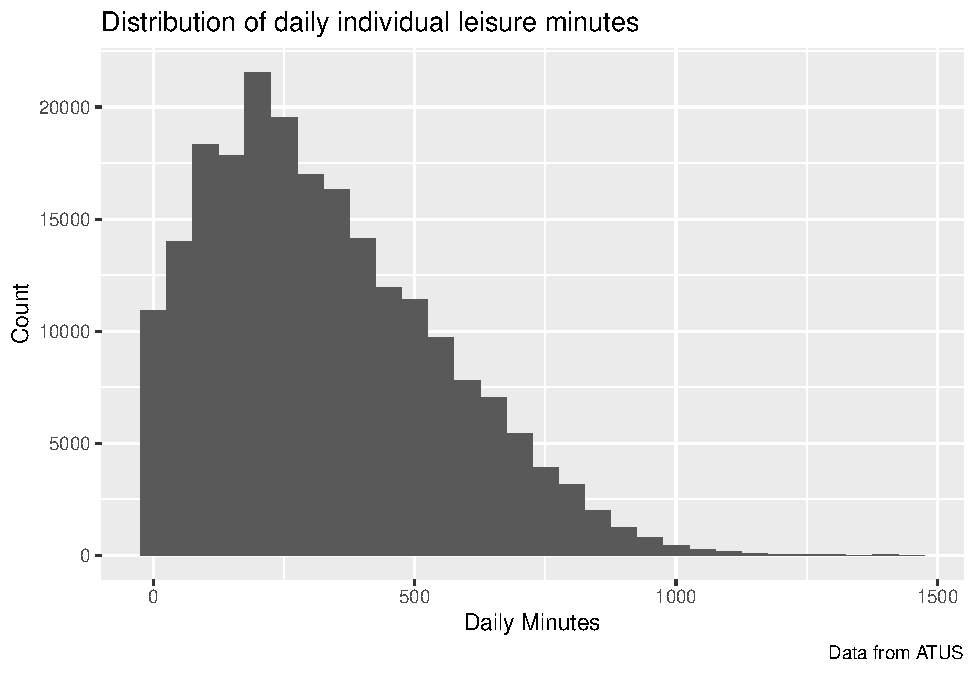
\includegraphics{Paper2_files/figure-latex/graphs-1.pdf}

\begin{Shaded}
\begin{Highlighting}[]
\NormalTok{csv }\SpecialCharTok{\%\textgreater{}\%}
  \FunctionTok{filter}\NormalTok{(year }\SpecialCharTok{\%in\%} \FunctionTok{c}\NormalTok{(}\DecValTok{2007}\NormalTok{, }\DecValTok{2009}\NormalTok{)) }\SpecialCharTok{\%\textgreater{}\%}
  \FunctionTok{ggplot}\NormalTok{(}\AttributeTok{mapping =} \FunctionTok{aes}\NormalTok{(}\AttributeTok{x =}\NormalTok{ bls\_leis)) }\SpecialCharTok{+}
  \FunctionTok{geom\_histogram}\NormalTok{(}\AttributeTok{binwidth=}\DecValTok{50}\NormalTok{) }\SpecialCharTok{+}
  \FunctionTok{facet\_wrap}\NormalTok{(}\SpecialCharTok{\textasciitilde{}}\NormalTok{year) }\SpecialCharTok{+}
  \FunctionTok{labs}\NormalTok{(}
  \AttributeTok{title =} \StringTok{"Distribution of daily individual leisure minutes"}\NormalTok{,}
  \AttributeTok{x =} \StringTok{"Daily Minutes"}\NormalTok{,}
  \AttributeTok{y =} \StringTok{"Count"}\NormalTok{,}
  \AttributeTok{caption =} \StringTok{"Data from ATUS"}\NormalTok{,}
\NormalTok{)}
\end{Highlighting}
\end{Shaded}

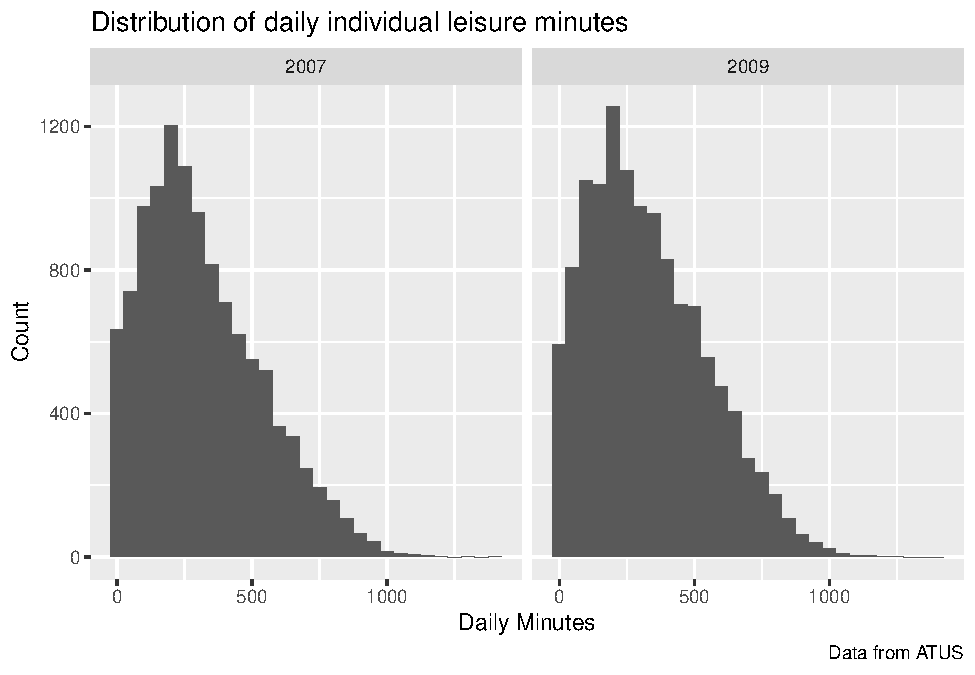
\includegraphics{Paper2_files/figure-latex/graphs-2.pdf}

\begin{Shaded}
\begin{Highlighting}[]
\CommentTok{\#leisure hours aggregate by gender}
\NormalTok{csv }\SpecialCharTok{\%\textgreater{}\%}
  \FunctionTok{group\_by}\NormalTok{(gender) }\SpecialCharTok{\%\textgreater{}\%}
  \FunctionTok{ggplot}\NormalTok{(}\AttributeTok{mapping =} \FunctionTok{aes}\NormalTok{(}\AttributeTok{x =}\NormalTok{ bls\_leis) )}\SpecialCharTok{+}
  \FunctionTok{geom\_histogram}\NormalTok{(}\AttributeTok{binwidth=}\DecValTok{50}\NormalTok{) }\SpecialCharTok{+}
  \FunctionTok{facet\_wrap}\NormalTok{(}\SpecialCharTok{\textasciitilde{}}\NormalTok{ gender) }\SpecialCharTok{+}
    \FunctionTok{labs}\NormalTok{(}
  \AttributeTok{title =} \StringTok{"Distribution of daily individual leisure minutes"}\NormalTok{,}
  \AttributeTok{x =} \StringTok{"Daily Minutes"}\NormalTok{,}
  \AttributeTok{y =} \StringTok{"Count"}\NormalTok{,}
  \AttributeTok{caption =} \StringTok{"Data from ATUS"}\NormalTok{,}
\NormalTok{)}
\end{Highlighting}
\end{Shaded}

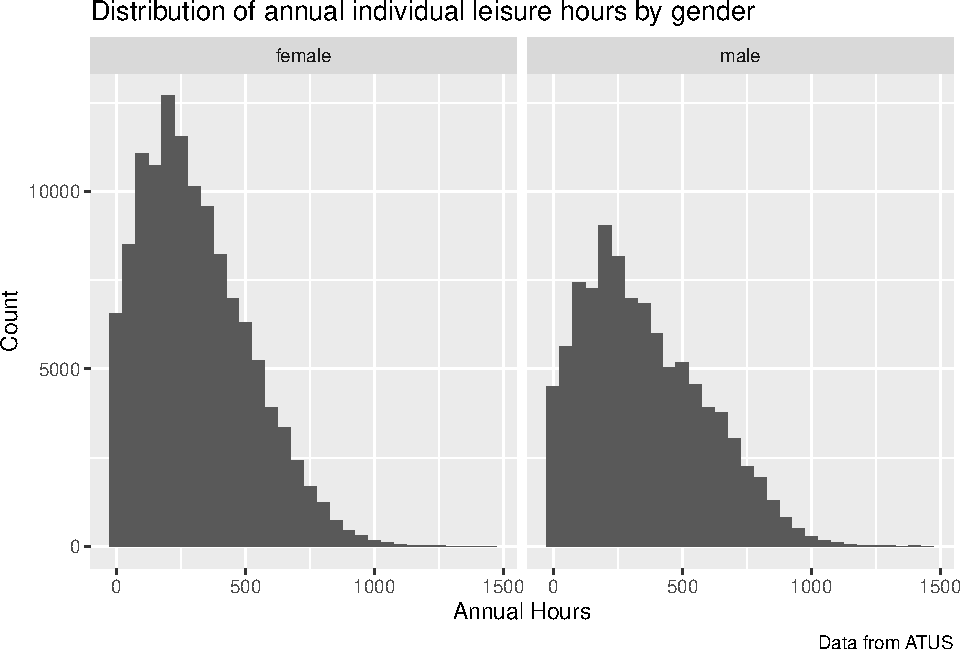
\includegraphics{Paper2_files/figure-latex/graphs-3.pdf}

\begin{Shaded}
\begin{Highlighting}[]
\NormalTok{csv }\SpecialCharTok{\%\textgreater{}\%}
  \FunctionTok{filter}\NormalTok{(year }\SpecialCharTok{\%in\%} \FunctionTok{c}\NormalTok{(}\DecValTok{2007}\NormalTok{, }\DecValTok{2009}\NormalTok{)) }\SpecialCharTok{\%\textgreater{}\%}
  \FunctionTok{ggplot}\NormalTok{(}\AttributeTok{mapping =} \FunctionTok{aes}\NormalTok{(}\AttributeTok{x =}\NormalTok{ bls\_leis)) }\SpecialCharTok{+}
  \FunctionTok{geom\_histogram}\NormalTok{(}\AttributeTok{binwidth=}\DecValTok{50}\NormalTok{) }\SpecialCharTok{+}
  \FunctionTok{facet\_wrap}\NormalTok{(}\SpecialCharTok{\textasciitilde{}}\NormalTok{ gender }\SpecialCharTok{+}\NormalTok{ year) }\SpecialCharTok{+}
  \FunctionTok{labs}\NormalTok{(}
  \AttributeTok{title =} \StringTok{"Distribution of daily individual leisure minutes"}\NormalTok{,}
  \AttributeTok{x =} \StringTok{"Daily Minutes"}\NormalTok{,}
  \AttributeTok{y =} \StringTok{"Count"}\NormalTok{,}
  \AttributeTok{caption =} \StringTok{"Data from ATUS"}\NormalTok{,}
\NormalTok{)}
\end{Highlighting}
\end{Shaded}

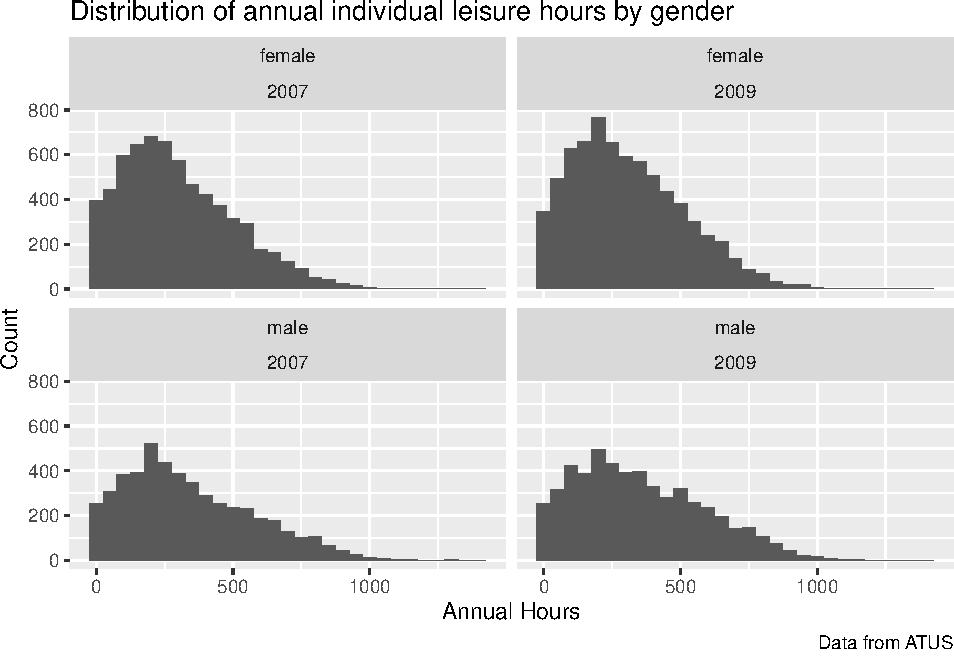
\includegraphics{Paper2_files/figure-latex/graphs-4.pdf}

\begin{Shaded}
\begin{Highlighting}[]
\CommentTok{\# Median}
\NormalTok{csv }\SpecialCharTok{\%\textgreater{}\%}
  \FunctionTok{group\_by}\NormalTok{(year, gender) }\SpecialCharTok{\%\textgreater{}\%}
  \FunctionTok{summarize}\NormalTok{(}\FunctionTok{median}\NormalTok{(bls\_leis)) }\SpecialCharTok{\%\textgreater{}\%}
  \FunctionTok{clean\_names}\NormalTok{() }\SpecialCharTok{\%\textgreater{}\%}
  \FunctionTok{ggplot}\NormalTok{(}\FunctionTok{aes}\NormalTok{(}\AttributeTok{x =}\NormalTok{ year, }\AttributeTok{y =}\NormalTok{ median\_bls\_leis)) }\SpecialCharTok{+}
  \FunctionTok{geom\_line}\NormalTok{() }\SpecialCharTok{+}
  \FunctionTok{facet\_wrap}\NormalTok{(}\SpecialCharTok{\textasciitilde{}}\NormalTok{ gender) }\SpecialCharTok{+}
  \FunctionTok{labs}\NormalTok{(}
  \AttributeTok{title =} \StringTok{"Median daily individual leisure minutes by gender"}\NormalTok{,}
  \AttributeTok{y =} \StringTok{"Daily Minutes"}\NormalTok{,}
  \AttributeTok{x =} \StringTok{"Year"}\NormalTok{,}
  \AttributeTok{caption =} \StringTok{"Data from ATUS"}\NormalTok{,}
\NormalTok{) }
\end{Highlighting}
\end{Shaded}

\begin{verbatim}
## `summarise()` has grouped output by 'year'. You can override using the
## `.groups` argument.
\end{verbatim}

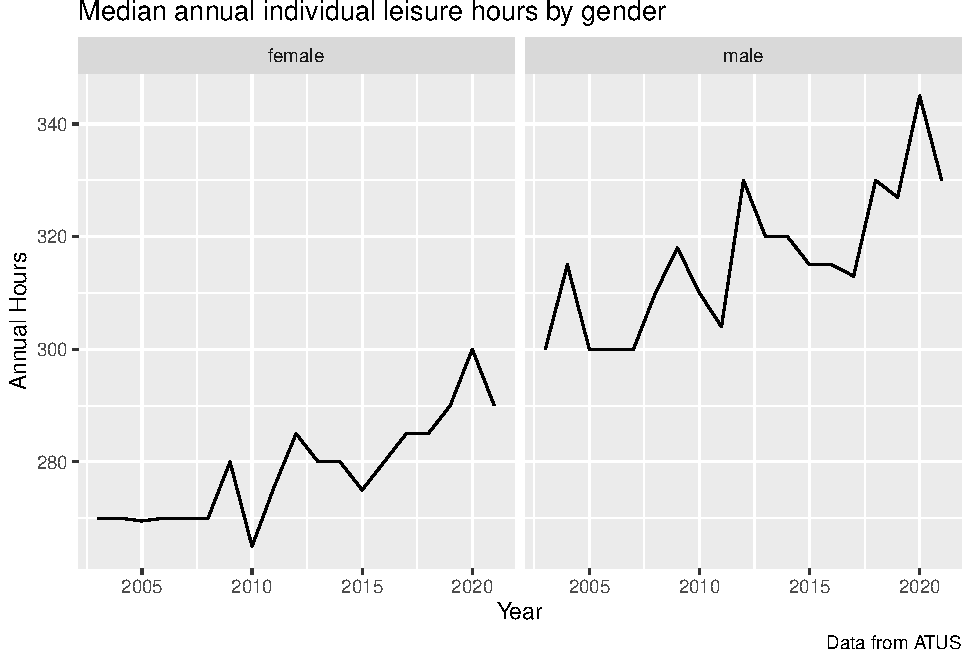
\includegraphics{Paper2_files/figure-latex/graphs-5.pdf}

\begin{Shaded}
\begin{Highlighting}[]
\CommentTok{\# Median }
\NormalTok{csv }\SpecialCharTok{\%\textgreater{}\%}
  \FunctionTok{filter}\NormalTok{(year }\SpecialCharTok{\textgreater{}} \DecValTok{2005}\NormalTok{) }\SpecialCharTok{\%\textgreater{}\%}
  \FunctionTok{filter}\NormalTok{(year }\SpecialCharTok{\textless{}} \DecValTok{2011}\NormalTok{) }\SpecialCharTok{\%\textgreater{}\%}
  \FunctionTok{group\_by}\NormalTok{(year, gender) }\SpecialCharTok{\%\textgreater{}\%}
  \FunctionTok{summarize}\NormalTok{(}\FunctionTok{median}\NormalTok{(bls\_leis)) }\SpecialCharTok{\%\textgreater{}\%}
  \FunctionTok{clean\_names}\NormalTok{() }\SpecialCharTok{\%\textgreater{}\%}
  \FunctionTok{ggplot}\NormalTok{(}\FunctionTok{aes}\NormalTok{(}\AttributeTok{x =}\NormalTok{ year, }\AttributeTok{y =}\NormalTok{ median\_bls\_leis)) }\SpecialCharTok{+}
  \FunctionTok{geom\_line}\NormalTok{() }\SpecialCharTok{+}
  \FunctionTok{facet\_wrap}\NormalTok{(}\SpecialCharTok{\textasciitilde{}}\NormalTok{ gender) }\SpecialCharTok{+}
  \FunctionTok{labs}\NormalTok{(}
  \AttributeTok{title =} \StringTok{"Median daily individual leisure minutes by gender"}\NormalTok{,}
  \AttributeTok{y =} \StringTok{"Daily Minutes"}\NormalTok{,}
  \AttributeTok{x =} \StringTok{"Year"}\NormalTok{,}
  \AttributeTok{caption =} \StringTok{"Data from ATUS"}\NormalTok{,}
\NormalTok{) }
\end{Highlighting}
\end{Shaded}

\begin{verbatim}
## `summarise()` has grouped output by 'year'. You can override using the
## `.groups` argument.
\end{verbatim}

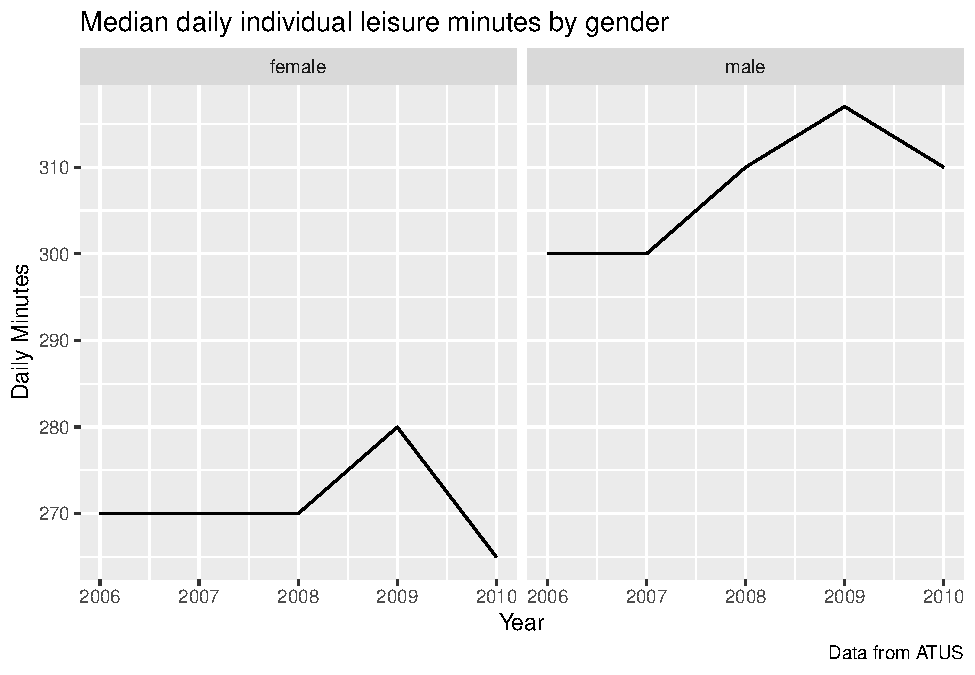
\includegraphics{Paper2_files/figure-latex/graphs-6.pdf}

\begin{Shaded}
\begin{Highlighting}[]
\CommentTok{\# Mean}
\NormalTok{csv }\SpecialCharTok{\%\textgreater{}\%}
  \FunctionTok{filter}\NormalTok{(year }\SpecialCharTok{\textgreater{}} \DecValTok{2005}\NormalTok{) }\SpecialCharTok{\%\textgreater{}\%}
  \FunctionTok{filter}\NormalTok{(year }\SpecialCharTok{\textless{}} \DecValTok{2011}\NormalTok{) }\SpecialCharTok{\%\textgreater{}\%}
  \FunctionTok{group\_by}\NormalTok{(year, gender) }\SpecialCharTok{\%\textgreater{}\%}
  \FunctionTok{summarize}\NormalTok{(}\FunctionTok{mean}\NormalTok{(bls\_leis)) }\SpecialCharTok{\%\textgreater{}\%}
  \FunctionTok{clean\_names}\NormalTok{() }\SpecialCharTok{\%\textgreater{}\%}
  \FunctionTok{ggplot}\NormalTok{(}\FunctionTok{aes}\NormalTok{(}\AttributeTok{x =}\NormalTok{ year, }\AttributeTok{y =}\NormalTok{ mean\_bls\_leis)) }\SpecialCharTok{+}
  \FunctionTok{geom\_line}\NormalTok{() }\SpecialCharTok{+}
  \FunctionTok{facet\_wrap}\NormalTok{(}\SpecialCharTok{\textasciitilde{}}\NormalTok{ gender) }\SpecialCharTok{+}
  \FunctionTok{labs}\NormalTok{(}
  \AttributeTok{title =} \StringTok{"Mean daily individual leisure minutes by gender"}\NormalTok{,}
  \AttributeTok{y =} \StringTok{"Daily Minutes"}\NormalTok{,}
  \AttributeTok{x =} \StringTok{"Year"}\NormalTok{,}
  \AttributeTok{caption =} \StringTok{"Data from ATUS"}\NormalTok{,}
\NormalTok{) }
\end{Highlighting}
\end{Shaded}

\begin{verbatim}
## `summarise()` has grouped output by 'year'. You can override using the
## `.groups` argument.
\end{verbatim}

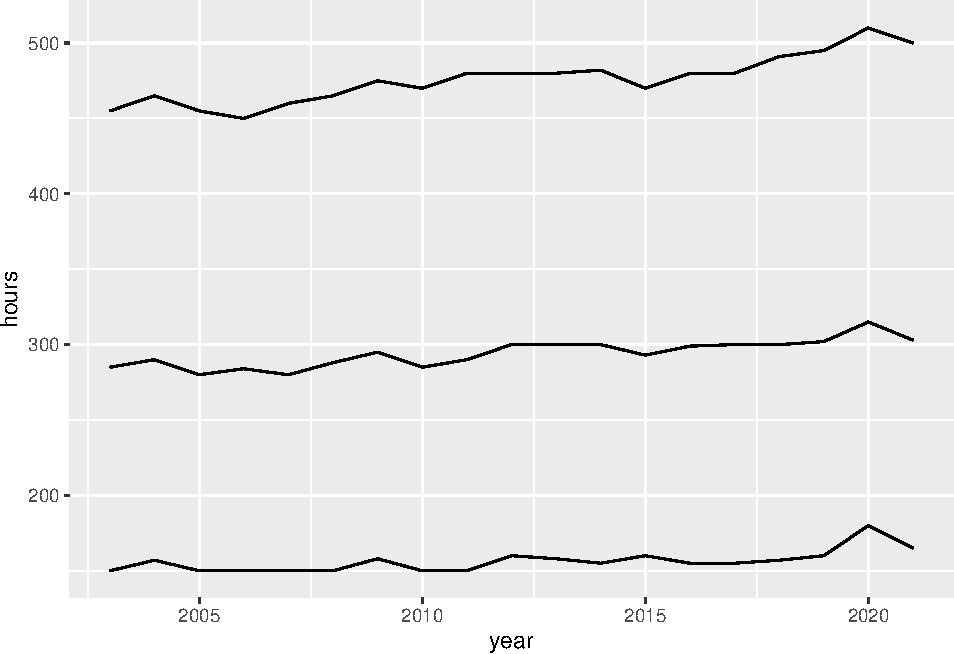
\includegraphics{Paper2_files/figure-latex/graphs-7.pdf}

\begin{Shaded}
\begin{Highlighting}[]
\CommentTok{\# All Quantile}
\NormalTok{csv }\SpecialCharTok{\%\textgreater{}\%}
  \FunctionTok{group\_by}\NormalTok{(year, gender) }\SpecialCharTok{\%\textgreater{}\%}
  \FunctionTok{summarize}\NormalTok{(}\AttributeTok{quantile\_25 =} \FunctionTok{quantile}\NormalTok{(bls\_leis, }\FloatTok{0.25}\NormalTok{), }\AttributeTok{quantile\_50 =} \FunctionTok{quantile}\NormalTok{(bls\_leis, }\FloatTok{0.5}\NormalTok{), }\AttributeTok{quantile\_75 =} \FunctionTok{quantile}\NormalTok{(bls\_leis, }\FloatTok{0.75}\NormalTok{)) }\SpecialCharTok{\%\textgreater{}\%}
  \FunctionTok{clean\_names}\NormalTok{() }\SpecialCharTok{\%\textgreater{}\%}
  \FunctionTok{pivot\_longer}\NormalTok{(quantile\_25}\SpecialCharTok{:}\NormalTok{quantile\_75, }\AttributeTok{names\_to =} \StringTok{"quantile"}\NormalTok{, }\AttributeTok{values\_to =} \StringTok{"hours"}\NormalTok{) }\SpecialCharTok{\%\textgreater{}\%}
  \FunctionTok{ggplot}\NormalTok{(}\FunctionTok{aes}\NormalTok{(}\AttributeTok{x =}\NormalTok{ year, }\AttributeTok{y =}\NormalTok{ hours, }\AttributeTok{group =}\NormalTok{ quantile, }\AttributeTok{colour =}\NormalTok{ quantile)) }\SpecialCharTok{+}
  \FunctionTok{geom\_line}\NormalTok{() }\SpecialCharTok{+}
    \FunctionTok{facet\_wrap}\NormalTok{(}\SpecialCharTok{\textasciitilde{}}\NormalTok{ gender) }\SpecialCharTok{+}
  \FunctionTok{labs}\NormalTok{(}
  \AttributeTok{title =} \StringTok{"Daily individual leisure minutes by gender"}\NormalTok{,}
  \AttributeTok{y =} \StringTok{"Daily Minutes"}\NormalTok{,}
  \AttributeTok{x =} \StringTok{"Year"}\NormalTok{,}
  \AttributeTok{caption =} \StringTok{"Data from ATUS"}\NormalTok{,}
\NormalTok{) }
\end{Highlighting}
\end{Shaded}

\begin{verbatim}
## `summarise()` has grouped output by 'year'. You can override using the
## `.groups` argument.
\end{verbatim}

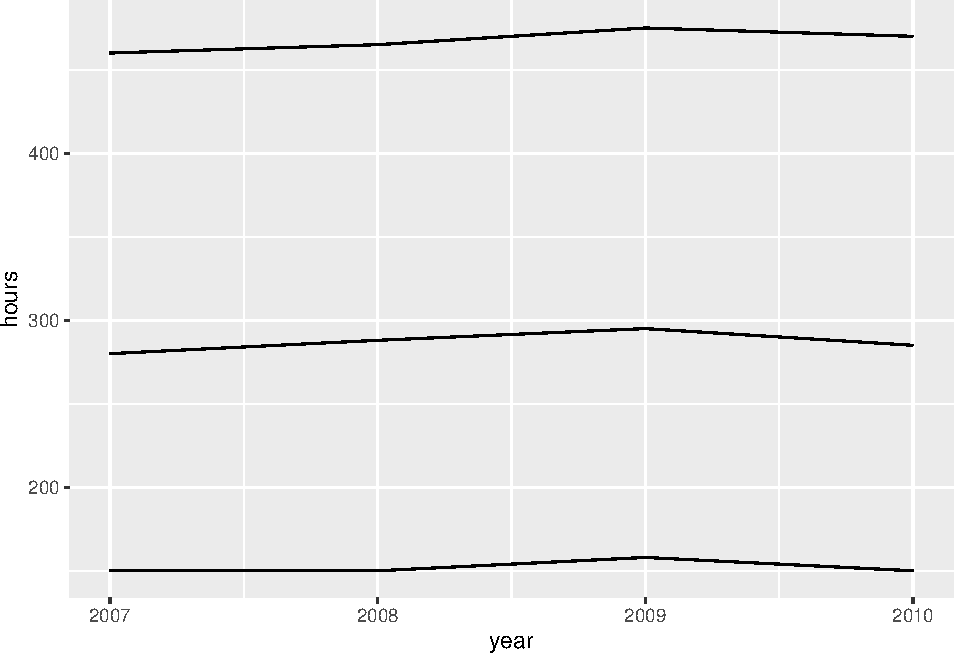
\includegraphics{Paper2_files/figure-latex/graphs-8.pdf}

\begin{Shaded}
\begin{Highlighting}[]
\NormalTok{csv }\SpecialCharTok{\%\textgreater{}\%}
  \FunctionTok{group\_by}\NormalTok{(year) }\SpecialCharTok{\%\textgreater{}\%}
  \FunctionTok{summarize}\NormalTok{(}\FunctionTok{quantile}\NormalTok{(bls\_leis, }\FloatTok{0.25}\NormalTok{), }\FunctionTok{quantile}\NormalTok{(bls\_leis, }\FloatTok{0.5}\NormalTok{), }\FunctionTok{quantile}\NormalTok{(bls\_leis, }\FloatTok{0.75}\NormalTok{)) }\SpecialCharTok{\%\textgreater{}\%}
  \FunctionTok{clean\_names}\NormalTok{() }\SpecialCharTok{\%\textgreater{}\%}
  \FunctionTok{pivot\_longer}\NormalTok{(}\SpecialCharTok{!}\NormalTok{year, }\AttributeTok{names\_to =} \StringTok{"quantile"}\NormalTok{, }\AttributeTok{values\_to =} \StringTok{"hours"}\NormalTok{) }\SpecialCharTok{\%\textgreater{}\%}
  \FunctionTok{ggplot}\NormalTok{(}\FunctionTok{aes}\NormalTok{(}\AttributeTok{x =}\NormalTok{ year, }\AttributeTok{y =}\NormalTok{ hours, }\AttributeTok{group =}\NormalTok{ quantile)) }\SpecialCharTok{+}
  \FunctionTok{geom\_line}\NormalTok{()}
\end{Highlighting}
\end{Shaded}

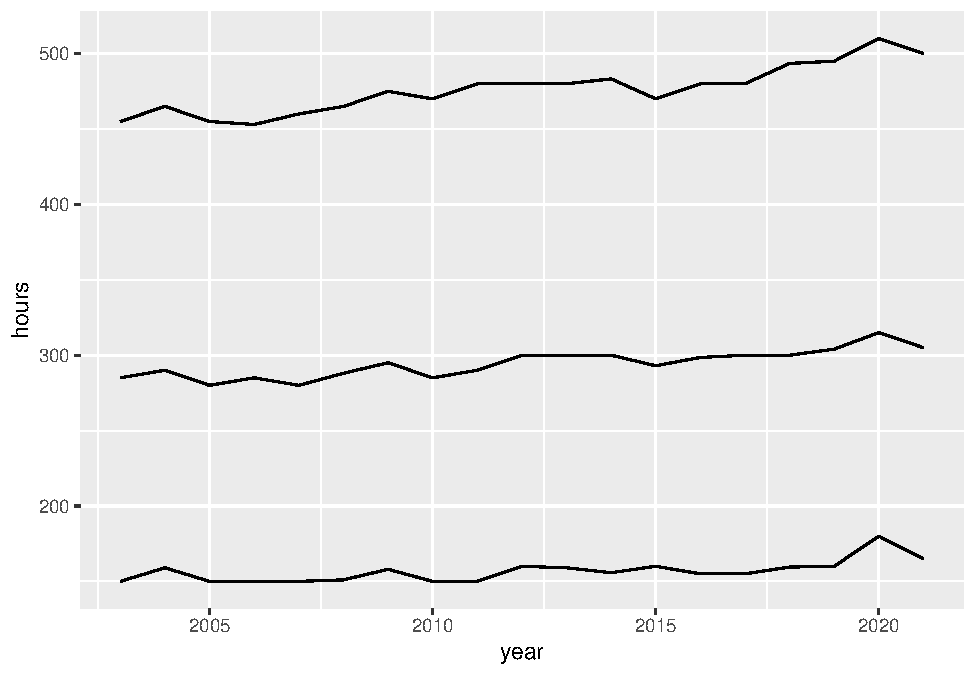
\includegraphics{Paper2_files/figure-latex/graphs-9.pdf}

\begin{Shaded}
\begin{Highlighting}[]
\NormalTok{csv }\SpecialCharTok{\%\textgreater{}\%}
  \FunctionTok{group\_by}\NormalTok{(year) }\SpecialCharTok{\%\textgreater{}\%}
  \FunctionTok{summarize}\NormalTok{(}\FunctionTok{quantile}\NormalTok{(bls\_leis, }\FloatTok{0.25}\NormalTok{), }\FunctionTok{quantile}\NormalTok{(bls\_leis, }\FloatTok{0.5}\NormalTok{), }\FunctionTok{quantile}\NormalTok{(bls\_leis, }\FloatTok{0.75}\NormalTok{)) }\SpecialCharTok{\%\textgreater{}\%}
  \FunctionTok{clean\_names}\NormalTok{() }\SpecialCharTok{\%\textgreater{}\%}
  \FunctionTok{pivot\_longer}\NormalTok{(}\SpecialCharTok{!}\NormalTok{year, }\AttributeTok{names\_to =} \StringTok{"quantile"}\NormalTok{, }\AttributeTok{values\_to =} \StringTok{"hours"}\NormalTok{) }\SpecialCharTok{\%\textgreater{}\%}
  \FunctionTok{filter}\NormalTok{(year }\SpecialCharTok{\textgreater{}} \DecValTok{2005}\NormalTok{) }\SpecialCharTok{\%\textgreater{}\%}
  \FunctionTok{filter}\NormalTok{(year }\SpecialCharTok{\textless{}} \DecValTok{2011}\NormalTok{) }\SpecialCharTok{\%\textgreater{}\%}
  \FunctionTok{ggplot}\NormalTok{(}\FunctionTok{aes}\NormalTok{(}\AttributeTok{x =}\NormalTok{ year, }\AttributeTok{y =}\NormalTok{ hours, }\AttributeTok{group =}\NormalTok{ quantile)) }\SpecialCharTok{+}
  \FunctionTok{geom\_line}\NormalTok{()}
\end{Highlighting}
\end{Shaded}

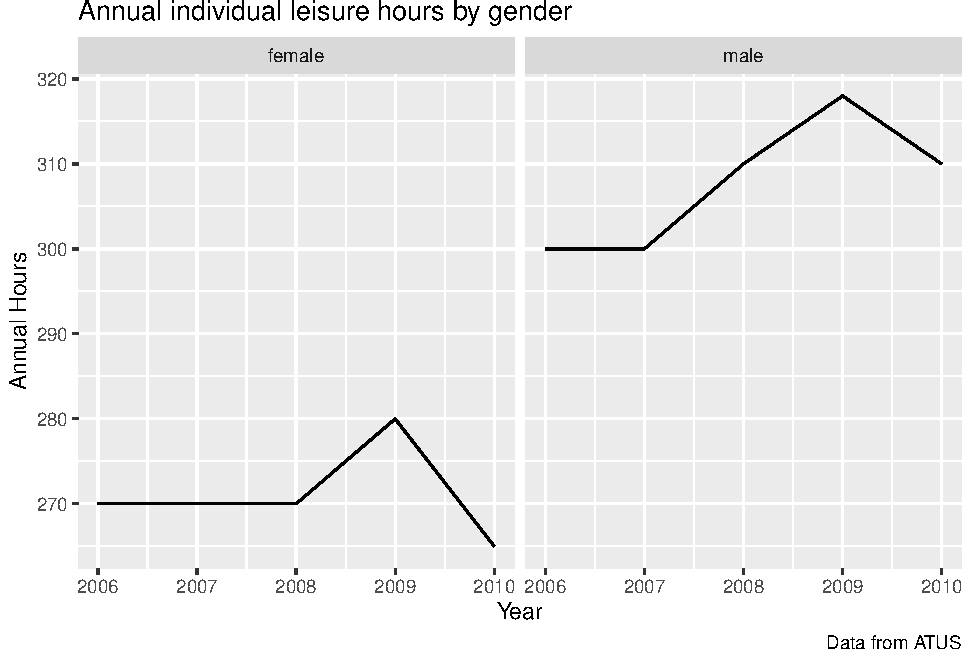
\includegraphics{Paper2_files/figure-latex/graphs-10.pdf}

\begin{Shaded}
\begin{Highlighting}[]
\CommentTok{\# by year, gender}
\NormalTok{csv }\SpecialCharTok{\%\textgreater{}\%}
  \FunctionTok{group\_by}\NormalTok{(year, gender) }\SpecialCharTok{\%\textgreater{}\%}
  \FunctionTok{summarize}\NormalTok{(}\AttributeTok{quantile\_25 =} \FunctionTok{quantile}\NormalTok{(bls\_leis, }\FloatTok{0.25}\NormalTok{), }\AttributeTok{quantile\_50 =} \FunctionTok{quantile}\NormalTok{(bls\_leis, }\FloatTok{0.5}\NormalTok{), }\AttributeTok{quantile\_75 =} \FunctionTok{quantile}\NormalTok{(bls\_leis, }\FloatTok{0.75}\NormalTok{)) }\SpecialCharTok{\%\textgreater{}\%}
  \FunctionTok{clean\_names}\NormalTok{() }\SpecialCharTok{\%\textgreater{}\%}
  \FunctionTok{pivot\_longer}\NormalTok{(quantile\_25}\SpecialCharTok{:}\NormalTok{quantile\_75, }\AttributeTok{names\_to =} \StringTok{"quantile"}\NormalTok{, }\AttributeTok{values\_to =} \StringTok{"hours"}\NormalTok{) }\SpecialCharTok{\%\textgreater{}\%}
  \FunctionTok{filter}\NormalTok{(year }\SpecialCharTok{\textgreater{}} \DecValTok{2005}\NormalTok{) }\SpecialCharTok{\%\textgreater{}\%}
  \FunctionTok{filter}\NormalTok{(year }\SpecialCharTok{\textless{}} \DecValTok{2011}\NormalTok{) }\SpecialCharTok{\%\textgreater{}\%}
  \FunctionTok{ggplot}\NormalTok{(}\FunctionTok{aes}\NormalTok{(}\AttributeTok{x =}\NormalTok{ year, }\AttributeTok{y =}\NormalTok{ hours, }\AttributeTok{group =}\NormalTok{ quantile, }\AttributeTok{colour =}\NormalTok{ quantile)) }\SpecialCharTok{+}
  \FunctionTok{geom\_line}\NormalTok{() }\SpecialCharTok{+}
  \FunctionTok{facet\_wrap}\NormalTok{(}\SpecialCharTok{\textasciitilde{}}\NormalTok{gender) }\SpecialCharTok{+}
    \FunctionTok{labs}\NormalTok{(}
  \AttributeTok{title =} \StringTok{"Daily individual leisure minutes by gender"}\NormalTok{,}
  \AttributeTok{y =} \StringTok{"Daily Minutes"}\NormalTok{,}
  \AttributeTok{x =} \StringTok{"Year"}\NormalTok{,}
  \AttributeTok{caption =} \StringTok{"Data from ATUS"}\NormalTok{,}
\NormalTok{) }
\end{Highlighting}
\end{Shaded}

\begin{verbatim}
## `summarise()` has grouped output by 'year'. You can override using the
## `.groups` argument.
\end{verbatim}

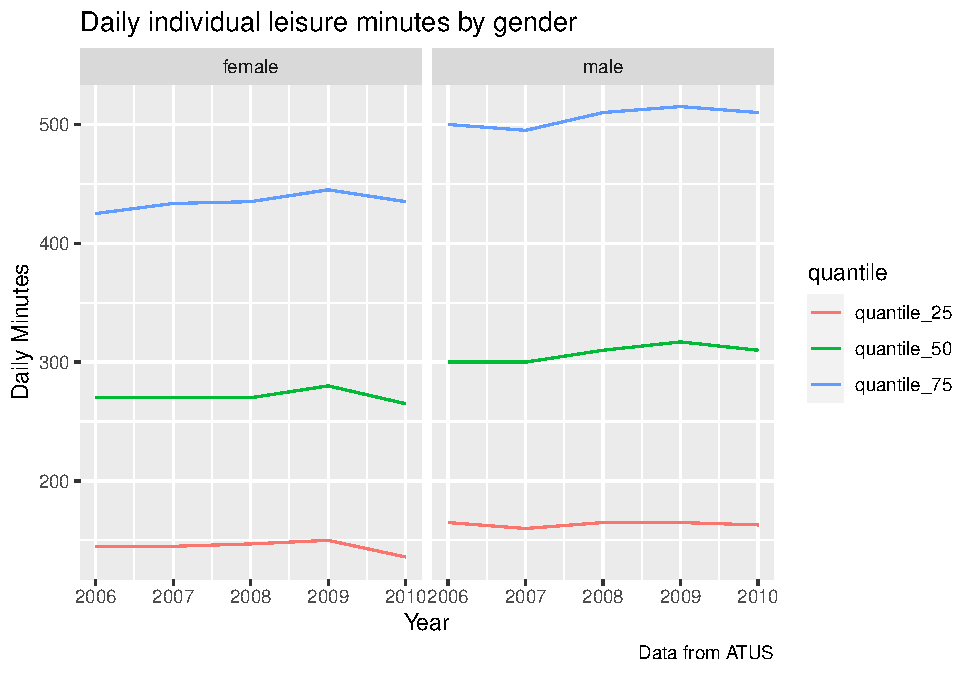
\includegraphics{Paper2_files/figure-latex/graphs-11.pdf}

\begin{Shaded}
\begin{Highlighting}[]
\CommentTok{\# by year, gender}
\NormalTok{csv }\SpecialCharTok{\%\textgreater{}\%}
  \FunctionTok{group\_by}\NormalTok{(year, gender) }\SpecialCharTok{\%\textgreater{}\%}
  \FunctionTok{summarize}\NormalTok{(}\AttributeTok{median =} \FunctionTok{median}\NormalTok{(bls\_leis)) }\SpecialCharTok{\%\textgreater{}\%}
  \FunctionTok{clean\_names}\NormalTok{() }\SpecialCharTok{\%\textgreater{}\%}
  \FunctionTok{filter}\NormalTok{(year }\SpecialCharTok{\textgreater{}} \DecValTok{2005}\NormalTok{) }\SpecialCharTok{\%\textgreater{}\%}
  \FunctionTok{filter}\NormalTok{(year }\SpecialCharTok{\textless{}} \DecValTok{2011}\NormalTok{) }\SpecialCharTok{\%\textgreater{}\%}
  \FunctionTok{ggplot}\NormalTok{(}\FunctionTok{aes}\NormalTok{(}\AttributeTok{x =}\NormalTok{ year, }\AttributeTok{y =}\NormalTok{ median)) }\SpecialCharTok{+}
  \FunctionTok{geom\_line}\NormalTok{() }\SpecialCharTok{+}
  \FunctionTok{facet\_wrap}\NormalTok{(}\SpecialCharTok{\textasciitilde{}}\NormalTok{gender) }\SpecialCharTok{+}
      \FunctionTok{labs}\NormalTok{(}
  \AttributeTok{title =} \StringTok{"Daily individual leisure minutes by gender"}\NormalTok{,}
  \AttributeTok{y =} \StringTok{"Daily Minutes"}\NormalTok{,}
  \AttributeTok{x =} \StringTok{"Year"}\NormalTok{,}
  \AttributeTok{caption =} \StringTok{"Data from ATUS"}\NormalTok{,}
\NormalTok{) }
\end{Highlighting}
\end{Shaded}

\begin{verbatim}
## `summarise()` has grouped output by 'year'. You can override using the
## `.groups` argument.
\end{verbatim}

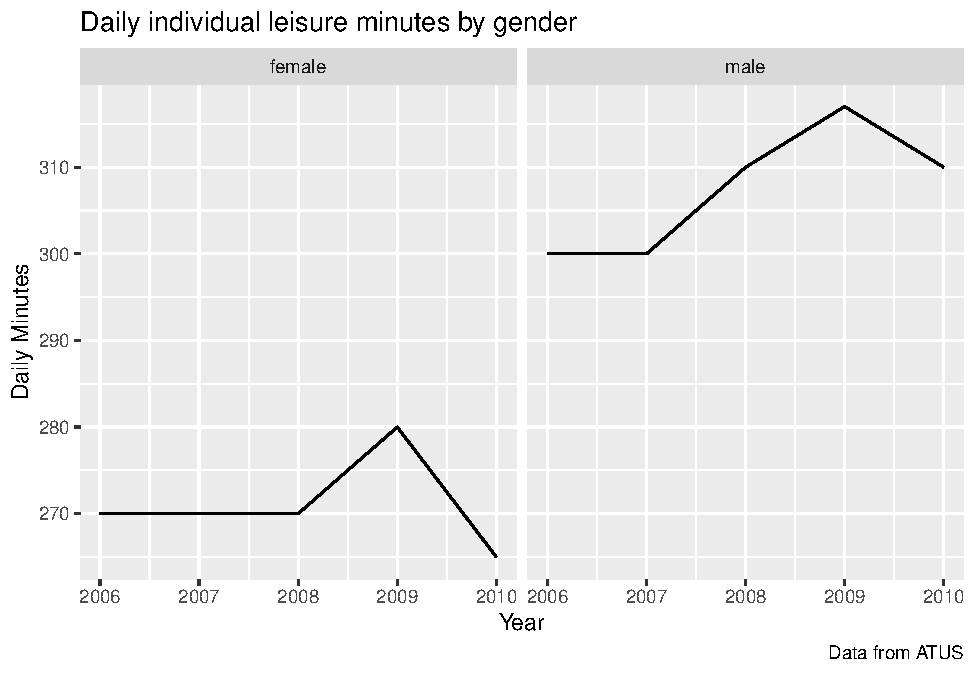
\includegraphics{Paper2_files/figure-latex/graphs-12.pdf}

\begin{Shaded}
\begin{Highlighting}[]
\CommentTok{\#csv \%\textgreater{}\%}
 \CommentTok{\# ggplot(mapping = aes(x = year, y = bls\_leis)) + }
 \CommentTok{\# geom\_jitter(alpha = 0.01)}
\end{Highlighting}
\end{Shaded}

\begin{Shaded}
\begin{Highlighting}[]
\CommentTok{\#naive regression of men versus women}
  

\NormalTok{g }\OtherTok{\textless{}{-}}\NormalTok{ csv }\SpecialCharTok{\%\textgreater{}\%}
  \FunctionTok{lm}\NormalTok{(}\AttributeTok{formula =}\NormalTok{ bls\_leis }\SpecialCharTok{\textasciitilde{}}\NormalTok{ gender)}

\CommentTok{\#naive regression of men versus women + year }

\NormalTok{y }\OtherTok{\textless{}{-}}\NormalTok{ csv }\SpecialCharTok{\%\textgreater{}\%}
  \FunctionTok{lm}\NormalTok{(}\AttributeTok{formula =}\NormalTok{ bls\_leis }\SpecialCharTok{\textasciitilde{}}\NormalTok{ gender }\SpecialCharTok{+}\NormalTok{ year)}

\CommentTok{\# race count}
\NormalTok{newcsv }\OtherTok{\textless{}{-}}\NormalTok{ csv }\SpecialCharTok{\%\textgreater{}\%}
 \FunctionTok{filter}\NormalTok{(race\_code }\SpecialCharTok{\textless{}=} \DecValTok{210}\NormalTok{)}

\NormalTok{newcsv}
\end{Highlighting}
\end{Shaded}

\begin{verbatim}
## # A tibble: 215,203 x 46
##     year  caseid pernum lineno        wt06  wt20 age   sex     race_code code_~1
##    <dbl>   <dbl>  <int> <int+lbl>    <dbl> <dbl> <dbl> <int+l> <dbl+lbl> <dbl+l>
##  1  2003 2.00e13      1 1         8155463.    NA 60    1 [Mal~ 110 [Bla~ 1 [Mar~
##  2  2003 2.00e13      1 1         1735323.    NA 41    2 [Fem~ 100 [Whi~ 1 [Mar~
##  3  2003 2.00e13      1 1         3830527.    NA 26    2 [Fem~ 100 [Whi~ 2 [Mar~
##  4  2003 2.00e13      1 1         6622023.    NA 36    2 [Fem~ 110 [Bla~ 1 [Mar~
##  5  2003 2.00e13      1 1         3068387.    NA 51    1 [Mal~ 100 [Whi~ 1 [Mar~
##  6  2003 2.00e13      1 1         3455425.    NA 32    2 [Fem~ 100 [Whi~ 4 [Div~
##  7  2003 2.00e13      1 1         1637826.    NA 44    2 [Fem~ 100 [Whi~ 3 [Wid~
##  8  2003 2.00e13      1 1         6574427.    NA 21    2 [Fem~ 100 [Whi~ 6 [Nev~
##  9  2003 2.00e13      1 1         1528296.    NA 33    2 [Fem~ 100 [Whi~ 1 [Mar~
## 10  2003 2.00e13      1 1         4277053.    NA 39    2 [Fem~ 110 [Bla~ 1 [Mar~
## # ... with 215,193 more rows, 36 more variables: code_education <dbl+lbl>,
## #   educyrs <int+lbl>, empstat_cps8 <dbl>, fullpart <int+lbl>, earnweek <dbl>,
## #   eldch <int+lbl>, yngch <int+lbl>, nchild <int+lbl>, bls_carehh <dbl>,
## #   bls_comm <dbl>, bls_educ <dbl>, bls_food <dbl>, bls_hhact <dbl>,
## #   bls_leis <dbl>, bls_leis_arts <dbl>, bls_leis_attend <dbl>,
## #   bls_leis_attsport <dbl>, bls_leis_partsport <dbl>, bls_leis_relax <dbl>,
## #   bls_leis_soc <dbl>, bls_leis_soccom <dbl>, bls_leis_soccomex <dbl>, ...
\end{verbatim}

\begin{Shaded}
\begin{Highlighting}[]
\NormalTok{newcsv }\SpecialCharTok{\%\textgreater{}\%}
  \FunctionTok{lm}\NormalTok{(}\AttributeTok{formula =}\NormalTok{ bls\_leis }\SpecialCharTok{\textasciitilde{}}\NormalTok{ gender }\SpecialCharTok{+}\NormalTok{ year }\SpecialCharTok{+}\NormalTok{ age }\SpecialCharTok{+}\NormalTok{ race) }
\end{Highlighting}
\end{Shaded}

\begin{verbatim}
## 
## Call:
## lm(formula = bls_leis ~ gender + year + age + race, data = .)
## 
## Coefficients:
##               (Intercept)                 gendermale  
##                 -619.9033                    49.6398  
##                      year                        age  
##                    0.3790                     3.6533  
##            raceAsian only             raceBlack only  
##                  -63.9127                    22.4987  
##            raceWhite only  raceWhite-American Indian  
##                  -20.1631                    -0.5827
\end{verbatim}

\begin{Shaded}
\begin{Highlighting}[]
\CommentTok{\# }
\NormalTok{a }\OtherTok{\textless{}{-}}\NormalTok{ newcsv }\SpecialCharTok{\%\textgreater{}\%}
  \FunctionTok{lm}\NormalTok{(}\AttributeTok{formula =}\NormalTok{ bls\_leis }\SpecialCharTok{\textasciitilde{}}\NormalTok{ gender }\SpecialCharTok{+}\NormalTok{ year }\SpecialCharTok{+}\NormalTok{ age }\SpecialCharTok{+}\NormalTok{ race) }
\FunctionTok{summary}\NormalTok{(a)}
\end{Highlighting}
\end{Shaded}

\begin{verbatim}
## 
## Call:
## lm(formula = bls_leis ~ gender + year + age + race, data = .)
## 
## Residuals:
##     Min      1Q  Median      3Q     Max 
## -521.52 -159.48  -31.18  135.19 1136.08 
## 
## Coefficients:
##                             Estimate Std. Error t value Pr(>|t|)    
## (Intercept)               -619.90327  168.42782  -3.681 0.000233 ***
## gendermale                  49.63976    0.92086  53.906  < 2e-16 ***
## year                         0.37904    0.08376   4.525 6.04e-06 ***
## age                          3.65328    0.02738 133.424  < 2e-16 ***
## raceAsian only             -63.91275    5.87182 -10.885  < 2e-16 ***
## raceBlack only              22.49865    5.48951   4.098 4.16e-05 ***
## raceWhite only             -20.16313    5.37329  -3.752 0.000175 ***
## raceWhite-American Indian   -0.58266    7.79477  -0.075 0.940413    
## ---
## Signif. codes:  0 '***' 0.001 '**' 0.01 '*' 0.05 '.' 0.1 ' ' 1
## 
## Residual standard error: 211.6 on 215195 degrees of freedom
## Multiple R-squared:  0.09465,    Adjusted R-squared:  0.09462 
## F-statistic:  3214 on 7 and 215195 DF,  p-value: < 2.2e-16
\end{verbatim}

\begin{Shaded}
\begin{Highlighting}[]
\NormalTok{newcsv}
\end{Highlighting}
\end{Shaded}

\begin{verbatim}
## # A tibble: 215,203 x 46
##     year  caseid pernum lineno        wt06  wt20 age   sex     race_code code_~1
##    <dbl>   <dbl>  <int> <int+lbl>    <dbl> <dbl> <dbl> <int+l> <dbl+lbl> <dbl+l>
##  1  2003 2.00e13      1 1         8155463.    NA 60    1 [Mal~ 110 [Bla~ 1 [Mar~
##  2  2003 2.00e13      1 1         1735323.    NA 41    2 [Fem~ 100 [Whi~ 1 [Mar~
##  3  2003 2.00e13      1 1         3830527.    NA 26    2 [Fem~ 100 [Whi~ 2 [Mar~
##  4  2003 2.00e13      1 1         6622023.    NA 36    2 [Fem~ 110 [Bla~ 1 [Mar~
##  5  2003 2.00e13      1 1         3068387.    NA 51    1 [Mal~ 100 [Whi~ 1 [Mar~
##  6  2003 2.00e13      1 1         3455425.    NA 32    2 [Fem~ 100 [Whi~ 4 [Div~
##  7  2003 2.00e13      1 1         1637826.    NA 44    2 [Fem~ 100 [Whi~ 3 [Wid~
##  8  2003 2.00e13      1 1         6574427.    NA 21    2 [Fem~ 100 [Whi~ 6 [Nev~
##  9  2003 2.00e13      1 1         1528296.    NA 33    2 [Fem~ 100 [Whi~ 1 [Mar~
## 10  2003 2.00e13      1 1         4277053.    NA 39    2 [Fem~ 110 [Bla~ 1 [Mar~
## # ... with 215,193 more rows, 36 more variables: code_education <dbl+lbl>,
## #   educyrs <int+lbl>, empstat_cps8 <dbl>, fullpart <int+lbl>, earnweek <dbl>,
## #   eldch <int+lbl>, yngch <int+lbl>, nchild <int+lbl>, bls_carehh <dbl>,
## #   bls_comm <dbl>, bls_educ <dbl>, bls_food <dbl>, bls_hhact <dbl>,
## #   bls_leis <dbl>, bls_leis_arts <dbl>, bls_leis_attend <dbl>,
## #   bls_leis_attsport <dbl>, bls_leis_partsport <dbl>, bls_leis_relax <dbl>,
## #   bls_leis_soc <dbl>, bls_leis_soccom <dbl>, bls_leis_soccomex <dbl>, ...
\end{verbatim}

\begin{Shaded}
\begin{Highlighting}[]
\CommentTok{\# education}
\NormalTok{newcsv1 }\OtherTok{\textless{}{-}}\NormalTok{ newcsv }\SpecialCharTok{\%\textgreater{}\%}
  \FunctionTok{mutate}\NormalTok{(}\AttributeTok{new\_educ =} \FunctionTok{ifelse}\NormalTok{(code\_education }\SpecialCharTok{\textless{}=} \DecValTok{17}\NormalTok{, }\StringTok{"\textless{}High School"}\NormalTok{, }\FunctionTok{ifelse}\NormalTok{(code\_education }\SpecialCharTok{\textgreater{}=} \DecValTok{40}\NormalTok{, }\StringTok{"\textgreater{}Four Year Degree"}\NormalTok{, }\StringTok{"High School Graduate"}\NormalTok{)))}
\NormalTok{  newcsv1}
\end{Highlighting}
\end{Shaded}

\begin{verbatim}
## # A tibble: 215,203 x 47
##     year  caseid pernum lineno        wt06  wt20 age   sex     race_code code_~1
##    <dbl>   <dbl>  <int> <int+lbl>    <dbl> <dbl> <dbl> <int+l> <dbl+lbl> <dbl+l>
##  1  2003 2.00e13      1 1         8155463.    NA 60    1 [Mal~ 110 [Bla~ 1 [Mar~
##  2  2003 2.00e13      1 1         1735323.    NA 41    2 [Fem~ 100 [Whi~ 1 [Mar~
##  3  2003 2.00e13      1 1         3830527.    NA 26    2 [Fem~ 100 [Whi~ 2 [Mar~
##  4  2003 2.00e13      1 1         6622023.    NA 36    2 [Fem~ 110 [Bla~ 1 [Mar~
##  5  2003 2.00e13      1 1         3068387.    NA 51    1 [Mal~ 100 [Whi~ 1 [Mar~
##  6  2003 2.00e13      1 1         3455425.    NA 32    2 [Fem~ 100 [Whi~ 4 [Div~
##  7  2003 2.00e13      1 1         1637826.    NA 44    2 [Fem~ 100 [Whi~ 3 [Wid~
##  8  2003 2.00e13      1 1         6574427.    NA 21    2 [Fem~ 100 [Whi~ 6 [Nev~
##  9  2003 2.00e13      1 1         1528296.    NA 33    2 [Fem~ 100 [Whi~ 1 [Mar~
## 10  2003 2.00e13      1 1         4277053.    NA 39    2 [Fem~ 110 [Bla~ 1 [Mar~
## # ... with 215,193 more rows, 37 more variables: code_education <dbl+lbl>,
## #   educyrs <int+lbl>, empstat_cps8 <dbl>, fullpart <int+lbl>, earnweek <dbl>,
## #   eldch <int+lbl>, yngch <int+lbl>, nchild <int+lbl>, bls_carehh <dbl>,
## #   bls_comm <dbl>, bls_educ <dbl>, bls_food <dbl>, bls_hhact <dbl>,
## #   bls_leis <dbl>, bls_leis_arts <dbl>, bls_leis_attend <dbl>,
## #   bls_leis_attsport <dbl>, bls_leis_partsport <dbl>, bls_leis_relax <dbl>,
## #   bls_leis_soc <dbl>, bls_leis_soccom <dbl>, bls_leis_soccomex <dbl>, ...
\end{verbatim}

\begin{Shaded}
\begin{Highlighting}[]
\NormalTok{b }\OtherTok{\textless{}{-}}\NormalTok{ newcsv1 }\SpecialCharTok{\%\textgreater{}\%}
  \FunctionTok{lm}\NormalTok{(}\AttributeTok{formula =}\NormalTok{ bls\_leis }\SpecialCharTok{\textasciitilde{}}\NormalTok{ gender }\SpecialCharTok{+}\NormalTok{ year }\SpecialCharTok{+}\NormalTok{ age }\SpecialCharTok{+}\NormalTok{ race }\SpecialCharTok{+}\NormalTok{ new\_educ) }
\FunctionTok{summary}\NormalTok{(b)}
\end{Highlighting}
\end{Shaded}

\begin{verbatim}
## 
## Call:
## lm(formula = bls_leis ~ gender + year + age + race + new_educ, 
##     data = .)
## 
## Residuals:
##     Min      1Q  Median      3Q     Max 
## -540.17 -157.13  -30.23  134.72 1126.00 
## 
## Coefficients:
##                                Estimate Std. Error t value Pr(>|t|)    
## (Intercept)                  -1.460e+03  1.680e+02  -8.690  < 2e-16 ***
## gendermale                    5.018e+01  9.148e-01  54.846  < 2e-16 ***
## year                          8.160e-01  8.360e-02   9.761  < 2e-16 ***
## age                           3.521e+00  2.734e-02 128.776  < 2e-16 ***
## raceAsian only               -3.772e+01  5.853e+00  -6.445 1.16e-10 ***
## raceBlack only                2.833e+01  5.454e+00   5.195 2.05e-07 ***
## raceWhite only               -7.820e+00  5.342e+00  -1.464    0.143    
## raceWhite-American Indian     5.327e+00  7.743e+00   0.688    0.491    
## new_educ>Four Year Degree    -7.570e+01  1.615e+00 -46.868  < 2e-16 ***
## new_educHigh School Graduate -3.247e+01  1.528e+00 -21.253  < 2e-16 ***
## ---
## Signif. codes:  0 '***' 0.001 '**' 0.01 '*' 0.05 '.' 0.1 ' ' 1
## 
## Residual standard error: 210.1 on 215193 degrees of freedom
## Multiple R-squared:  0.1068, Adjusted R-squared:  0.1068 
## F-statistic:  2859 on 9 and 215193 DF,  p-value: < 2.2e-16
\end{verbatim}

\begin{Shaded}
\begin{Highlighting}[]
\NormalTok{newcsv1}
\end{Highlighting}
\end{Shaded}

\begin{verbatim}
## # A tibble: 215,203 x 47
##     year  caseid pernum lineno        wt06  wt20 age   sex     race_code code_~1
##    <dbl>   <dbl>  <int> <int+lbl>    <dbl> <dbl> <dbl> <int+l> <dbl+lbl> <dbl+l>
##  1  2003 2.00e13      1 1         8155463.    NA 60    1 [Mal~ 110 [Bla~ 1 [Mar~
##  2  2003 2.00e13      1 1         1735323.    NA 41    2 [Fem~ 100 [Whi~ 1 [Mar~
##  3  2003 2.00e13      1 1         3830527.    NA 26    2 [Fem~ 100 [Whi~ 2 [Mar~
##  4  2003 2.00e13      1 1         6622023.    NA 36    2 [Fem~ 110 [Bla~ 1 [Mar~
##  5  2003 2.00e13      1 1         3068387.    NA 51    1 [Mal~ 100 [Whi~ 1 [Mar~
##  6  2003 2.00e13      1 1         3455425.    NA 32    2 [Fem~ 100 [Whi~ 4 [Div~
##  7  2003 2.00e13      1 1         1637826.    NA 44    2 [Fem~ 100 [Whi~ 3 [Wid~
##  8  2003 2.00e13      1 1         6574427.    NA 21    2 [Fem~ 100 [Whi~ 6 [Nev~
##  9  2003 2.00e13      1 1         1528296.    NA 33    2 [Fem~ 100 [Whi~ 1 [Mar~
## 10  2003 2.00e13      1 1         4277053.    NA 39    2 [Fem~ 110 [Bla~ 1 [Mar~
## # ... with 215,193 more rows, 37 more variables: code_education <dbl+lbl>,
## #   educyrs <int+lbl>, empstat_cps8 <dbl>, fullpart <int+lbl>, earnweek <dbl>,
## #   eldch <int+lbl>, yngch <int+lbl>, nchild <int+lbl>, bls_carehh <dbl>,
## #   bls_comm <dbl>, bls_educ <dbl>, bls_food <dbl>, bls_hhact <dbl>,
## #   bls_leis <dbl>, bls_leis_arts <dbl>, bls_leis_attend <dbl>,
## #   bls_leis_attsport <dbl>, bls_leis_partsport <dbl>, bls_leis_relax <dbl>,
## #   bls_leis_soc <dbl>, bls_leis_soccom <dbl>, bls_leis_soccomex <dbl>, ...
\end{verbatim}

\begin{Shaded}
\begin{Highlighting}[]
\CommentTok{\# with children}
 

\NormalTok{c }\OtherTok{\textless{}{-}}\NormalTok{ newcsv1 }\SpecialCharTok{\%\textgreater{}\%}
  \FunctionTok{lm}\NormalTok{(}\AttributeTok{formula =}\NormalTok{ bls\_leis }\SpecialCharTok{\textasciitilde{}}\NormalTok{ gender }\SpecialCharTok{+}\NormalTok{ year }\SpecialCharTok{+}\NormalTok{ age }\SpecialCharTok{+}\NormalTok{ race }\SpecialCharTok{+}\NormalTok{ new\_educ }\SpecialCharTok{+}\NormalTok{ nchild) }
\FunctionTok{summary}\NormalTok{(c)}
\end{Highlighting}
\end{Shaded}

\begin{verbatim}
## 
## Call:
## lm(formula = bls_leis ~ gender + year + age + race + new_educ + 
##     nchild, data = .)
## 
## Residuals:
##     Min      1Q  Median      3Q     Max 
## -539.78 -154.29  -28.94  133.49 1119.88 
## 
## Coefficients:
##                                Estimate Std. Error t value Pr(>|t|)    
## (Intercept)                  -1.163e+03  1.665e+02  -6.987 2.82e-12 ***
## gendermale                    4.746e+01  9.070e-01  52.328  < 2e-16 ***
## year                          7.017e-01  8.281e-02   8.475  < 2e-16 ***
## age                           2.805e+00  2.923e-02  95.957  < 2e-16 ***
## raceAsian only               -3.909e+01  5.796e+00  -6.744 1.55e-11 ***
## raceBlack only                2.045e+01  5.402e+00   3.785 0.000154 ***
## raceWhite only               -1.061e+01  5.291e+00  -2.005 0.044918 *  
## raceWhite-American Indian     1.367e-01  7.669e+00   0.018 0.985777    
## new_educ>Four Year Degree    -7.829e+01  1.600e+00 -48.929  < 2e-16 ***
## new_educHigh School Graduate -3.766e+01  1.515e+00 -24.856  < 2e-16 ***
## nchild                       -2.817e+01  4.332e-01 -65.015  < 2e-16 ***
## ---
## Signif. codes:  0 '***' 0.001 '**' 0.01 '*' 0.05 '.' 0.1 ' ' 1
## 
## Residual standard error: 208.1 on 215192 degrees of freedom
## Multiple R-squared:  0.124,  Adjusted R-squared:  0.124 
## F-statistic:  3046 on 10 and 215192 DF,  p-value: < 2.2e-16
\end{verbatim}

\begin{Shaded}
\begin{Highlighting}[]
\CommentTok{\#marital status}

\NormalTok{d }\OtherTok{\textless{}{-}}\NormalTok{ newcsv1 }\SpecialCharTok{\%\textgreater{}\%}
  \FunctionTok{lm}\NormalTok{(}\AttributeTok{formula =}\NormalTok{ bls\_leis }\SpecialCharTok{\textasciitilde{}}\NormalTok{ gender }\SpecialCharTok{+}\NormalTok{ year }\SpecialCharTok{+}\NormalTok{ age }\SpecialCharTok{+}\NormalTok{ race }\SpecialCharTok{+}\NormalTok{ new\_educ }\SpecialCharTok{+}\NormalTok{ nchild }\SpecialCharTok{+}\NormalTok{ marst\_simple) }
\FunctionTok{summary}\NormalTok{(d)}
\end{Highlighting}
\end{Shaded}

\begin{verbatim}
## 
## Call:
## lm(formula = bls_leis ~ gender + year + age + race + new_educ + 
##     nchild + marst_simple, data = .)
## 
## Residuals:
##     Min      1Q  Median      3Q     Max 
## -559.43 -153.49  -28.26  133.29 1112.50 
## 
## Coefficients:
##                                  Estimate Std. Error t value Pr(>|t|)    
## (Intercept)                    -823.13997  166.26341  -4.951 7.40e-07 ***
## gendermale                       49.21853    0.91265  53.929  < 2e-16 ***
## year                              0.50959    0.08276   6.158 7.39e-10 ***
## age                               3.16991    0.03366  94.166  < 2e-16 ***
## raceAsian only                  -32.02787    5.78311  -5.538 3.06e-08 ***
## raceBlack only                   16.43517    5.38740   3.051  0.00228 ** 
## raceWhite only                   -6.52156    5.27602  -1.236  0.21643    
## raceWhite-American Indian         2.39392    7.64590   0.313  0.75421    
## new_educ>Four Year Degree       -72.82025    1.60459 -45.383  < 2e-16 ***
## new_educHigh School Graduate    -34.86904    1.51239 -23.056  < 2e-16 ***
## nchild                          -21.25080    0.47340 -44.889  < 2e-16 ***
## marst_simpleNever Married        46.67237    1.35601  34.419  < 2e-16 ***
## marst_simpleSeparated/Divorced   22.66065    1.15216  19.668  < 2e-16 ***
## ---
## Signif. codes:  0 '***' 0.001 '**' 0.01 '*' 0.05 '.' 0.1 ' ' 1
## 
## Residual standard error: 207.5 on 215190 degrees of freedom
## Multiple R-squared:  0.1293, Adjusted R-squared:  0.1292 
## F-statistic:  2663 on 12 and 215190 DF,  p-value: < 2.2e-16
\end{verbatim}

\begin{Shaded}
\begin{Highlighting}[]
\FunctionTok{stargazer}\NormalTok{(a, b, c, d, }\AttributeTok{title=}\StringTok{"Various Models"}\NormalTok{, }\AttributeTok{align=}\ConstantTok{TRUE}\NormalTok{, }\AttributeTok{type =} \StringTok{"text"}\NormalTok{)}
\end{Highlighting}
\end{Shaded}

\begin{verbatim}
## 
## Various Models
## ========================================================================================================================================================
##                                                                                   Dependent variable:                                                   
##                                -------------------------------------------------------------------------------------------------------------------------
##                                                                                        bls_leis                                                         
##                                             (1)                           (2)                           (3)                            (4)              
## --------------------------------------------------------------------------------------------------------------------------------------------------------
## gendermale                               49.640***                     50.175***                     47.459***                      49.219***           
##                                           (0.921)                       (0.915)                       (0.907)                        (0.913)            
##                                                                                                                                                         
## year                                     0.379***                      0.816***                       0.702***                       0.510***           
##                                           (0.084)                       (0.084)                       (0.083)                        (0.083)            
##                                                                                                                                                         
## age                                      3.653***                      3.521***                       2.805***                       3.170***           
##                                           (0.027)                       (0.027)                       (0.029)                        (0.034)            
##                                                                                                                                                         
## raceAsian only                          -63.913***                    -37.723***                     -39.090***                     -32.028***          
##                                           (5.872)                       (5.853)                       (5.796)                        (5.783)            
##                                                                                                                                                         
## raceBlack only                           22.499***                     28.330***                     20.450***                      16.435***           
##                                           (5.490)                       (5.454)                       (5.402)                        (5.387)            
##                                                                                                                                                         
## raceWhite only                          -20.163***                      -7.820                       -10.610**                        -6.522            
##                                           (5.373)                       (5.342)                       (5.291)                        (5.276)            
##                                                                                                                                                         
## raceWhite-American Indian                 -0.583                         5.327                         0.137                          2.394             
##                                           (7.795)                       (7.743)                       (7.669)                        (7.646)            
##                                                                                                                                                         
## new_educ> Four Year Degree                                            -75.705***                     -78.293***                     -72.820***          
##                                                                         (1.615)                       (1.600)                        (1.605)            
##                                                                                                                                                         
## new_educHigh School Graduate                                          -32.466***                     -37.656***                     -34.869***          
##                                                                         (1.528)                       (1.515)                        (1.512)            
##                                                                                                                                                         
## nchild                                                                                               -28.166***                     -21.251***          
##                                                                                                       (0.433)                        (0.473)            
##                                                                                                                                                         
## marst_simpleNever Married                                                                                                           46.672***           
##                                                                                                                                      (1.356)            
##                                                                                                                                                         
## marst_simpleSeparated/Divorced                                                                                                      22.661***           
##                                                                                                                                      (1.152)            
##                                                                                                                                                         
## Constant                                -619.903***                  -1,460.115***                 -1,162.998***                   -823.140***          
##                                          (168.428)                     (168.014)                     (166.451)                      (166.263)           
##                                                                                                                                                         
## --------------------------------------------------------------------------------------------------------------------------------------------------------
## Observations                              215,203                       215,203                       215,203                        215,203            
## R2                                         0.095                         0.107                         0.124                          0.129             
## Adjusted R2                                0.095                         0.107                         0.124                          0.129             
## Residual Std. Error                211.569 (df = 215195)         210.144 (df = 215193)         208.111 (df = 215192)          207.483 (df = 215190)     
## F Statistic                    3,213.841*** (df = 7; 215195) 2,859.141*** (df = 9; 215193) 3,046.454*** (df = 10; 215192) 2,662.895*** (df = 12; 215190)
## ========================================================================================================================================================
## Note:                                                                                                                        *p<0.1; **p<0.05; ***p<0.01
\end{verbatim}

\begin{Shaded}
\begin{Highlighting}[]
\NormalTok{newcsv1 }\SpecialCharTok{\%\textgreater{}\%}
  \FunctionTok{filter}\NormalTok{(year }\SpecialCharTok{\textgreater{}} \DecValTok{2006}\NormalTok{) }\SpecialCharTok{\%\textgreater{}\%}
  \FunctionTok{filter}\NormalTok{(year }\SpecialCharTok{\textless{}} \DecValTok{2011}\NormalTok{) }\SpecialCharTok{\%\textgreater{}\%}
  \FunctionTok{group\_by}\NormalTok{(year) }\SpecialCharTok{\%\textgreater{}\%}
  \FunctionTok{count}\NormalTok{(emp) }\SpecialCharTok{\%\textgreater{}\%}
  \FunctionTok{filter}\NormalTok{(emp }\SpecialCharTok{==} \StringTok{"Unemployed"}\NormalTok{) }\SpecialCharTok{\%\textgreater{}\%}
  \FunctionTok{ggplot}\NormalTok{(}\AttributeTok{mapping =} \FunctionTok{aes}\NormalTok{(}\AttributeTok{x =}\NormalTok{ year, }\AttributeTok{y =}\NormalTok{ n)) }\SpecialCharTok{+}
  \FunctionTok{geom\_line}\NormalTok{() }\SpecialCharTok{+}
  \FunctionTok{labs}\NormalTok{(}
  \AttributeTok{title =} \StringTok{"Unemployment"}\NormalTok{,}
  \AttributeTok{y =} \StringTok{"Daily Minutes"}\NormalTok{,}
  \AttributeTok{x =} \StringTok{"Count"}\NormalTok{,}
  \AttributeTok{caption =} \StringTok{"Data from ATUS"}\NormalTok{,}
\NormalTok{)}
\end{Highlighting}
\end{Shaded}

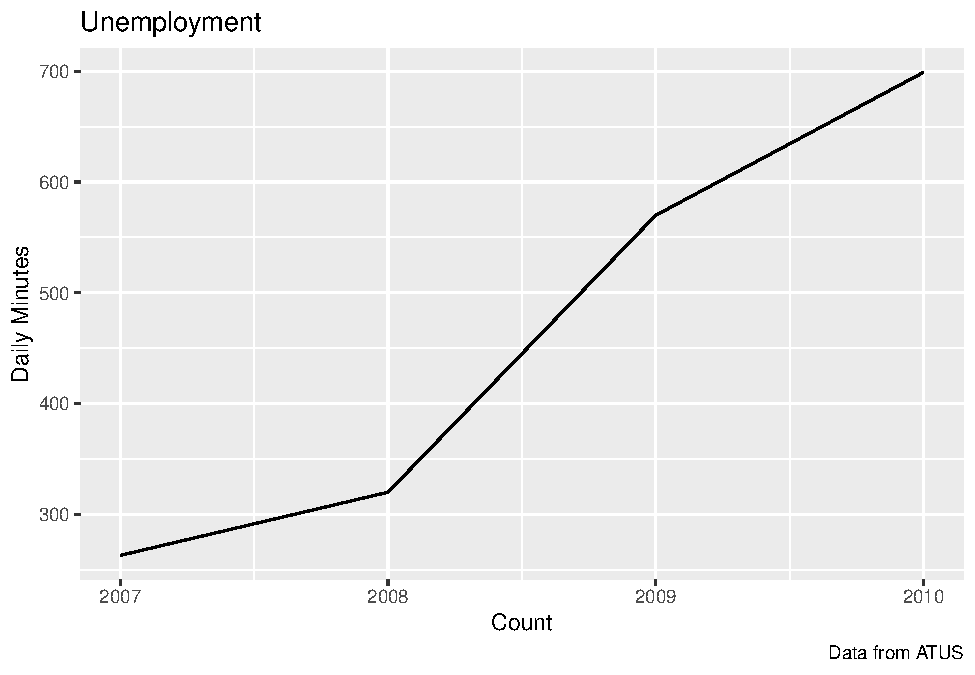
\includegraphics{Paper2_files/figure-latex/employment-1.pdf}

\begin{Shaded}
\begin{Highlighting}[]
  \CommentTok{\#facet\_wrap(\textasciitilde{}emp)}

\NormalTok{newcsv1 }\SpecialCharTok{\%\textgreater{}\%}
  \FunctionTok{ggplot}\NormalTok{(}\AttributeTok{mapping =} \FunctionTok{aes}\NormalTok{(}\AttributeTok{x =}\NormalTok{ bls\_leis)) }\SpecialCharTok{+}
  \FunctionTok{geom\_histogram}\NormalTok{() }\SpecialCharTok{+}
  \FunctionTok{facet\_wrap}\NormalTok{(}\SpecialCharTok{\textasciitilde{}}\NormalTok{emp)}
\end{Highlighting}
\end{Shaded}

\begin{verbatim}
## `stat_bin()` using `bins = 30`. Pick better value with `binwidth`.
\end{verbatim}

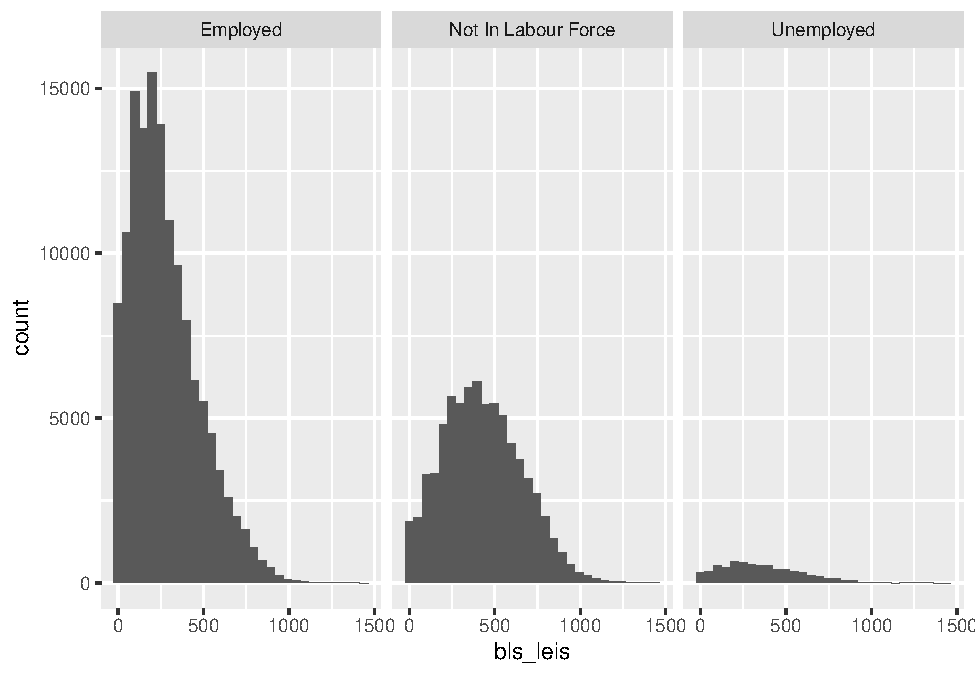
\includegraphics{Paper2_files/figure-latex/employment-2.pdf}

\begin{Shaded}
\begin{Highlighting}[]
\NormalTok{newcsv1 }\SpecialCharTok{\%\textgreater{}\%}
  \FunctionTok{group\_by}\NormalTok{(emp, gender, new\_educ, year) }\SpecialCharTok{\%\textgreater{}\%}
  \FunctionTok{summarize}\NormalTok{(}\AttributeTok{median =} \FunctionTok{median}\NormalTok{(bls\_leis)) }\SpecialCharTok{\%\textgreater{}\%}
  \FunctionTok{ggplot}\NormalTok{(}\AttributeTok{mapping =} \FunctionTok{aes}\NormalTok{(}\AttributeTok{x =}\NormalTok{ year, }\AttributeTok{y =}\NormalTok{ median, }\AttributeTok{group =}\NormalTok{ new\_educ, }\AttributeTok{colour =}\NormalTok{ new\_educ)) }\SpecialCharTok{+}
  \FunctionTok{geom\_line}\NormalTok{() }\SpecialCharTok{+}
  \FunctionTok{facet\_wrap}\NormalTok{(}\SpecialCharTok{\textasciitilde{}}\NormalTok{gender }\SpecialCharTok{+}\NormalTok{ emp) }\SpecialCharTok{+}
  \FunctionTok{labs}\NormalTok{(}
  \AttributeTok{title =} \StringTok{"Daily individual leisure minutes"}\NormalTok{,}
  \AttributeTok{y =} \StringTok{"Daily Minutes"}\NormalTok{,}
  \AttributeTok{x =} \StringTok{"Count"}\NormalTok{,}
  \AttributeTok{caption =} \StringTok{"Data from ATUS"}\NormalTok{,}
\NormalTok{)}
\end{Highlighting}
\end{Shaded}

\begin{verbatim}
## `summarise()` has grouped output by 'emp', 'gender', 'new_educ'. You can
## override using the `.groups` argument.
\end{verbatim}

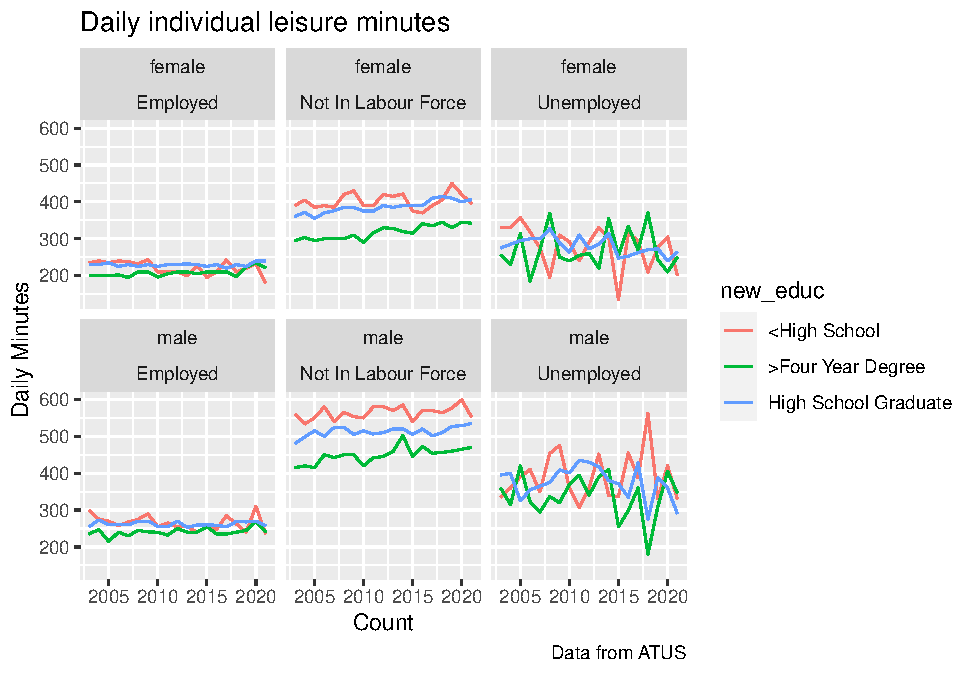
\includegraphics{Paper2_files/figure-latex/employment-3.pdf}

\begin{Shaded}
\begin{Highlighting}[]
\NormalTok{newcsv1 }\SpecialCharTok{\%\textgreater{}\%}
  \FunctionTok{filter}\NormalTok{(year }\SpecialCharTok{\textgreater{}} \DecValTok{2006}\NormalTok{) }\SpecialCharTok{\%\textgreater{}\%}
  \FunctionTok{filter}\NormalTok{(year }\SpecialCharTok{\textless{}} \DecValTok{2011}\NormalTok{) }\SpecialCharTok{\%\textgreater{}\%}
  \FunctionTok{group\_by}\NormalTok{(emp, gender, new\_educ, year) }\SpecialCharTok{\%\textgreater{}\%}
  \FunctionTok{summarize}\NormalTok{(}\AttributeTok{median =} \FunctionTok{median}\NormalTok{(bls\_leis)) }\SpecialCharTok{\%\textgreater{}\%}
  \FunctionTok{ggplot}\NormalTok{(}\AttributeTok{mapping =} \FunctionTok{aes}\NormalTok{(}\AttributeTok{x =}\NormalTok{ year, }\AttributeTok{y =}\NormalTok{ median, }\AttributeTok{group =}\NormalTok{ new\_educ, }\AttributeTok{colour =}\NormalTok{ new\_educ)) }\SpecialCharTok{+}
  \FunctionTok{geom\_line}\NormalTok{() }\SpecialCharTok{+}
  \FunctionTok{facet\_wrap}\NormalTok{(}\SpecialCharTok{\textasciitilde{}}\NormalTok{gender }\SpecialCharTok{+}\NormalTok{ emp) }\SpecialCharTok{+}
  \FunctionTok{labs}\NormalTok{(}
  \AttributeTok{title =} \StringTok{"Daily individual leisure minutes"}\NormalTok{,}
  \AttributeTok{y =} \StringTok{"Daily Minutes"}\NormalTok{,}
  \AttributeTok{x =} \StringTok{"Count"}\NormalTok{,}
  \AttributeTok{caption =} \StringTok{"Data from ATUS"}\NormalTok{,}
\NormalTok{)}
\end{Highlighting}
\end{Shaded}

\begin{verbatim}
## `summarise()` has grouped output by 'emp', 'gender', 'new_educ'. You can
## override using the `.groups` argument.
\end{verbatim}

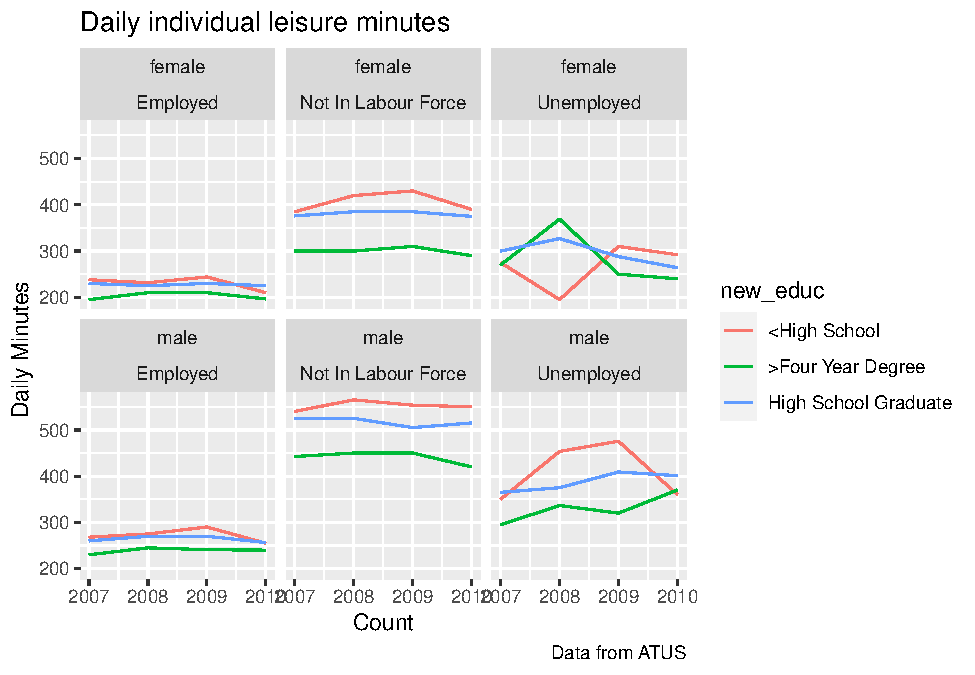
\includegraphics{Paper2_files/figure-latex/employment-4.pdf}

\begin{Shaded}
\begin{Highlighting}[]
\NormalTok{newcsv1 }\SpecialCharTok{\%\textgreater{}\%}
  \FunctionTok{filter}\NormalTok{(year }\SpecialCharTok{\textgreater{}} \DecValTok{2006}\NormalTok{) }\SpecialCharTok{\%\textgreater{}\%}
  \FunctionTok{filter}\NormalTok{(year }\SpecialCharTok{\textless{}} \DecValTok{2011}\NormalTok{) }\SpecialCharTok{\%\textgreater{}\%}
  \FunctionTok{group\_by}\NormalTok{(emp, gender) }\SpecialCharTok{\%\textgreater{}\%}
  \FunctionTok{tally}\NormalTok{()}
\end{Highlighting}
\end{Shaded}

\begin{verbatim}
## # A tibble: 6 x 3
## # Groups:   emp [3]
##   emp                 gender     n
##   <chr>               <chr>  <int>
## 1 Employed            female 15763
## 2 Employed            male   14996
## 3 Not In Labour Force female 10591
## 4 Not In Labour Force male    4855
## 5 Unemployed          female   959
## 6 Unemployed          male     893
\end{verbatim}

\begin{Shaded}
\begin{Highlighting}[]
\NormalTok{newcsv1 }\SpecialCharTok{\%\textgreater{}\%}
  \FunctionTok{filter}\NormalTok{(year }\SpecialCharTok{\textgreater{}} \DecValTok{2006}\NormalTok{) }\SpecialCharTok{\%\textgreater{}\%}
  \FunctionTok{filter}\NormalTok{(year }\SpecialCharTok{\textless{}} \DecValTok{2011}\NormalTok{) }\SpecialCharTok{\%\textgreater{}\%}
  \FunctionTok{group\_by}\NormalTok{(emp, year) }\SpecialCharTok{\%\textgreater{}\%}
  \FunctionTok{tally}\NormalTok{() }\SpecialCharTok{\%\textgreater{}\%}
  \FunctionTok{pivot\_wider}\NormalTok{(}\AttributeTok{names\_from =}\NormalTok{ year, }\AttributeTok{values\_from =}\NormalTok{ n) }\SpecialCharTok{\%\textgreater{}\%}
  \FunctionTok{clean\_names}\NormalTok{() }\SpecialCharTok{\%\textgreater{}\%}
  \FunctionTok{mutate}\NormalTok{(}\AttributeTok{change\_2008 =}\NormalTok{ x2008}\SpecialCharTok{{-}}\NormalTok{x2007) }\SpecialCharTok{\%\textgreater{}\%}
  \FunctionTok{mutate}\NormalTok{(}\AttributeTok{change\_2009 =}\NormalTok{ x2009}\SpecialCharTok{{-}}\NormalTok{x2008) }\SpecialCharTok{\%\textgreater{}\%}
  \FunctionTok{mutate}\NormalTok{(}\AttributeTok{change\_2010 =}\NormalTok{ x2010}\SpecialCharTok{{-}}\NormalTok{x2009) }\SpecialCharTok{\%\textgreater{}\%}
  \FunctionTok{select}\NormalTok{(}\DecValTok{1}\NormalTok{, }\DecValTok{6}\SpecialCharTok{:}\DecValTok{8}\NormalTok{)}
\end{Highlighting}
\end{Shaded}

\begin{verbatim}
## # A tibble: 3 x 4
## # Groups:   emp [3]
##   emp                 change_2008 change_2009 change_2010
##   <chr>                     <int>       <int>       <int>
## 1 Employed                    305          -3         -70
## 2 Not In Labour Force         111         241           7
## 3 Unemployed                   57         250         129
\end{verbatim}

\begin{Shaded}
\begin{Highlighting}[]
\CommentTok{\#Change}

\NormalTok{change }\OtherTok{\textless{}{-}}\NormalTok{ newcsv1 }\SpecialCharTok{\%\textgreater{}\%}
  \FunctionTok{group\_by}\NormalTok{(gender,  year, new\_educ, child, marst\_simple) }\SpecialCharTok{\%\textgreater{}\%}
  \FunctionTok{summarize}\NormalTok{(}\FunctionTok{median}\NormalTok{(bls\_leis)) }\SpecialCharTok{\%\textgreater{}\%}
  \FunctionTok{clean\_names}\NormalTok{() }\SpecialCharTok{\%\textgreater{}\%}
  \FunctionTok{pivot\_wider}\NormalTok{(}\AttributeTok{values\_from =}\NormalTok{ median\_bls\_leis, }\AttributeTok{names\_from =}\NormalTok{ year) }\SpecialCharTok{\%\textgreater{}\%}
  \FunctionTok{clean\_names}\NormalTok{() }\SpecialCharTok{\%\textgreater{}\%}
  \FunctionTok{mutate}\NormalTok{(}\AttributeTok{leisure\_change =}\NormalTok{ x2009 }\SpecialCharTok{{-}}\NormalTok{ x2007)}
\end{Highlighting}
\end{Shaded}

\begin{verbatim}
## `summarise()` has grouped output by 'gender', 'year', 'new_educ', 'child'. You
## can override using the `.groups` argument.
\end{verbatim}

\begin{Shaded}
\begin{Highlighting}[]
\NormalTok{change11 }\OtherTok{\textless{}{-}}\NormalTok{ newcsv1 }\SpecialCharTok{\%\textgreater{}\%}
  \FunctionTok{group\_by}\NormalTok{(gender,  year, new\_educ, child, marst\_simple, emp) }\SpecialCharTok{\%\textgreater{}\%}
  \FunctionTok{summarize}\NormalTok{(}\FunctionTok{median}\NormalTok{(bls\_leis)) }\SpecialCharTok{\%\textgreater{}\%}
  \FunctionTok{clean\_names}\NormalTok{() }\SpecialCharTok{\%\textgreater{}\%}
  \FunctionTok{pivot\_wider}\NormalTok{(}\AttributeTok{values\_from =}\NormalTok{ median\_bls\_leis, }\AttributeTok{names\_from =}\NormalTok{ year) }\SpecialCharTok{\%\textgreater{}\%}
  \FunctionTok{clean\_names}\NormalTok{() }\SpecialCharTok{\%\textgreater{}\%}
  \FunctionTok{mutate}\NormalTok{(}\AttributeTok{leisure\_change =}\NormalTok{ x2009 }\SpecialCharTok{{-}}\NormalTok{ x2007)}
\end{Highlighting}
\end{Shaded}

\begin{verbatim}
## `summarise()` has grouped output by 'gender', 'year', 'new_educ', 'child',
## 'marst_simple'. You can override using the `.groups` argument.
\end{verbatim}

\begin{Shaded}
\begin{Highlighting}[]
\NormalTok{change2 }\OtherTok{\textless{}{-}}\NormalTok{ newcsv1 }\SpecialCharTok{\%\textgreater{}\%}
  \FunctionTok{group\_by}\NormalTok{(gender, year) }\SpecialCharTok{\%\textgreater{}\%}
  \FunctionTok{summarize}\NormalTok{(}\FunctionTok{median}\NormalTok{(bls\_leis)) }\SpecialCharTok{\%\textgreater{}\%}
  \FunctionTok{clean\_names}\NormalTok{() }\SpecialCharTok{\%\textgreater{}\%}
  \FunctionTok{pivot\_wider}\NormalTok{(}\AttributeTok{values\_from =}\NormalTok{ median\_bls\_leis, }\AttributeTok{names\_from =}\NormalTok{ year) }\SpecialCharTok{\%\textgreater{}\%}
  \FunctionTok{clean\_names}\NormalTok{() }\SpecialCharTok{\%\textgreater{}\%}
  \FunctionTok{mutate}\NormalTok{(}\AttributeTok{leisure\_change =}\NormalTok{ x2009 }\SpecialCharTok{{-}}\NormalTok{ x2007)}
\end{Highlighting}
\end{Shaded}

\begin{verbatim}
## `summarise()` has grouped output by 'gender'. You can override using the
## `.groups` argument.
\end{verbatim}

\begin{Shaded}
\begin{Highlighting}[]
\NormalTok{change3 }\OtherTok{\textless{}{-}}\NormalTok{ newcsv1 }\SpecialCharTok{\%\textgreater{}\%}
  \FunctionTok{group\_by}\NormalTok{(gender,  year, new\_educ, nchild, marst\_simple) }\SpecialCharTok{\%\textgreater{}\%}
  \FunctionTok{summarize}\NormalTok{(}\FunctionTok{median}\NormalTok{(bls\_leis)) }\SpecialCharTok{\%\textgreater{}\%}
  \FunctionTok{clean\_names}\NormalTok{() }\SpecialCharTok{\%\textgreater{}\%}
  \FunctionTok{pivot\_wider}\NormalTok{(}\AttributeTok{values\_from =}\NormalTok{ median\_bls\_leis, }\AttributeTok{names\_from =}\NormalTok{ year) }\SpecialCharTok{\%\textgreater{}\%}
  \FunctionTok{clean\_names}\NormalTok{() }\SpecialCharTok{\%\textgreater{}\%}
  \FunctionTok{mutate}\NormalTok{(}\AttributeTok{leisure\_change =}\NormalTok{ x2009 }\SpecialCharTok{{-}}\NormalTok{ x2007)}
\end{Highlighting}
\end{Shaded}

\begin{verbatim}
## `summarise()` has grouped output by 'gender', 'year', 'new_educ', 'nchild'. You
## can override using the `.groups` argument.
\end{verbatim}

\begin{Shaded}
\begin{Highlighting}[]
\NormalTok{change4 }\OtherTok{\textless{}{-}}\NormalTok{ newcsv1 }\SpecialCharTok{\%\textgreater{}\%}
  \FunctionTok{group\_by}\NormalTok{(gender,  year, new\_educ, nchild, marst\_simple) }\SpecialCharTok{\%\textgreater{}\%}
  \FunctionTok{summarize}\NormalTok{(}\FunctionTok{mean}\NormalTok{(bls\_leis)) }\SpecialCharTok{\%\textgreater{}\%}
  \FunctionTok{clean\_names}\NormalTok{() }\SpecialCharTok{\%\textgreater{}\%}
  \FunctionTok{pivot\_wider}\NormalTok{(}\AttributeTok{values\_from =}\NormalTok{ mean\_bls\_leis, }\AttributeTok{names\_from =}\NormalTok{ year) }\SpecialCharTok{\%\textgreater{}\%}
  \FunctionTok{clean\_names}\NormalTok{() }\SpecialCharTok{\%\textgreater{}\%}
  \FunctionTok{mutate}\NormalTok{(}\AttributeTok{leisure\_change =}\NormalTok{ x2009 }\SpecialCharTok{{-}}\NormalTok{ x2007)}
\end{Highlighting}
\end{Shaded}

\begin{verbatim}
## `summarise()` has grouped output by 'gender', 'year', 'new_educ', 'nchild'. You
## can override using the `.groups` argument.
\end{verbatim}

\begin{Shaded}
\begin{Highlighting}[]
\NormalTok{change12 }\OtherTok{\textless{}{-}}\NormalTok{ newcsv1 }\SpecialCharTok{\%\textgreater{}\%}
  \FunctionTok{group\_by}\NormalTok{(gender,  year, emp) }\SpecialCharTok{\%\textgreater{}\%}
  \FunctionTok{summarize}\NormalTok{(}\FunctionTok{median}\NormalTok{(bls\_leis)) }\SpecialCharTok{\%\textgreater{}\%}
  \FunctionTok{clean\_names}\NormalTok{() }\SpecialCharTok{\%\textgreater{}\%}
  \FunctionTok{pivot\_wider}\NormalTok{(}\AttributeTok{values\_from =}\NormalTok{ median\_bls\_leis, }\AttributeTok{names\_from =}\NormalTok{ year) }\SpecialCharTok{\%\textgreater{}\%}
  \FunctionTok{clean\_names}\NormalTok{() }\SpecialCharTok{\%\textgreater{}\%}
  \FunctionTok{mutate}\NormalTok{(}\AttributeTok{leisure\_change =}\NormalTok{ x2009 }\SpecialCharTok{{-}}\NormalTok{ x2007)}
\end{Highlighting}
\end{Shaded}

\begin{verbatim}
## `summarise()` has grouped output by 'gender', 'year'. You can override using
## the `.groups` argument.
\end{verbatim}

\begin{Shaded}
\begin{Highlighting}[]
\CommentTok{\#child}
\NormalTok{newcsv1}
\end{Highlighting}
\end{Shaded}

\begin{verbatim}
## # A tibble: 215,203 x 47
##     year  caseid pernum lineno        wt06  wt20 age   sex     race_code code_~1
##    <dbl>   <dbl>  <int> <int+lbl>    <dbl> <dbl> <dbl> <int+l> <dbl+lbl> <dbl+l>
##  1  2003 2.00e13      1 1         8155463.    NA 60    1 [Mal~ 110 [Bla~ 1 [Mar~
##  2  2003 2.00e13      1 1         1735323.    NA 41    2 [Fem~ 100 [Whi~ 1 [Mar~
##  3  2003 2.00e13      1 1         3830527.    NA 26    2 [Fem~ 100 [Whi~ 2 [Mar~
##  4  2003 2.00e13      1 1         6622023.    NA 36    2 [Fem~ 110 [Bla~ 1 [Mar~
##  5  2003 2.00e13      1 1         3068387.    NA 51    1 [Mal~ 100 [Whi~ 1 [Mar~
##  6  2003 2.00e13      1 1         3455425.    NA 32    2 [Fem~ 100 [Whi~ 4 [Div~
##  7  2003 2.00e13      1 1         1637826.    NA 44    2 [Fem~ 100 [Whi~ 3 [Wid~
##  8  2003 2.00e13      1 1         6574427.    NA 21    2 [Fem~ 100 [Whi~ 6 [Nev~
##  9  2003 2.00e13      1 1         1528296.    NA 33    2 [Fem~ 100 [Whi~ 1 [Mar~
## 10  2003 2.00e13      1 1         4277053.    NA 39    2 [Fem~ 110 [Bla~ 1 [Mar~
## # ... with 215,193 more rows, 37 more variables: code_education <dbl+lbl>,
## #   educyrs <int+lbl>, empstat_cps8 <dbl>, fullpart <int+lbl>, earnweek <dbl>,
## #   eldch <int+lbl>, yngch <int+lbl>, nchild <int+lbl>, bls_carehh <dbl>,
## #   bls_comm <dbl>, bls_educ <dbl>, bls_food <dbl>, bls_hhact <dbl>,
## #   bls_leis <dbl>, bls_leis_arts <dbl>, bls_leis_attend <dbl>,
## #   bls_leis_attsport <dbl>, bls_leis_partsport <dbl>, bls_leis_relax <dbl>,
## #   bls_leis_soc <dbl>, bls_leis_soccom <dbl>, bls_leis_soccomex <dbl>, ...
\end{verbatim}

\begin{Shaded}
\begin{Highlighting}[]
\NormalTok{delta }\OtherTok{\textless{}{-}}\NormalTok{ change }\SpecialCharTok{\%\textgreater{}\%}
  \FunctionTok{lm}\NormalTok{(}\AttributeTok{formula =}\NormalTok{ leisure\_change }\SpecialCharTok{\textasciitilde{}}\NormalTok{ gender}\SpecialCharTok{+}\NormalTok{ new\_educ}\SpecialCharTok{+}\NormalTok{ child}\SpecialCharTok{+}\NormalTok{ marst\_simple)}
\FunctionTok{summary}\NormalTok{(delta)}
\end{Highlighting}
\end{Shaded}

\begin{verbatim}
## 
## Call:
## lm(formula = leisure_change ~ gender + new_educ + child + marst_simple, 
##     data = .)
## 
## Residuals:
##     Min      1Q  Median      3Q     Max 
## -79.986 -28.778  -3.104  17.799 148.194 
## 
## Coefficients:
##                                Estimate Std. Error t value Pr(>|t|)  
## (Intercept)                      25.597     23.737   1.078   0.2898  
## gendermale                       17.111     17.943   0.954   0.3482  
## new_educ>Four Year Degree       -34.667     21.976  -1.577   0.1255  
## new_educHigh School Graduate    -47.875     21.976  -2.179   0.0376 *
## child                             8.389     17.943   0.468   0.6436  
## marst_simpleNever Married        20.875     21.976   0.950   0.3500  
## marst_simpleSeparated/Divorced   32.208     21.976   1.466   0.1535  
## ---
## Signif. codes:  0 '***' 0.001 '**' 0.01 '*' 0.05 '.' 0.1 ' ' 1
## 
## Residual standard error: 53.83 on 29 degrees of freedom
## Multiple R-squared:  0.2247, Adjusted R-squared:  0.06423 
## F-statistic:   1.4 on 6 and 29 DF,  p-value: 0.2481
\end{verbatim}

\begin{Shaded}
\begin{Highlighting}[]
\NormalTok{delta11 }\OtherTok{\textless{}{-}}\NormalTok{ change11 }\SpecialCharTok{\%\textgreater{}\%}
  \FunctionTok{lm}\NormalTok{(}\AttributeTok{formula =}\NormalTok{ leisure\_change }\SpecialCharTok{\textasciitilde{}}\NormalTok{ gender}\SpecialCharTok{+}\NormalTok{ new\_educ}\SpecialCharTok{+}\NormalTok{ child}\SpecialCharTok{+}\NormalTok{ marst\_simple }\SpecialCharTok{+}\NormalTok{ emp)}
\FunctionTok{summary}\NormalTok{(delta11)}
\end{Highlighting}
\end{Shaded}

\begin{verbatim}
## 
## Call:
## lm(formula = leisure_change ~ gender + new_educ + child + marst_simple + 
##     emp, data = .)
## 
## Residuals:
##     Min      1Q  Median      3Q     Max 
## -406.53  -41.12   -3.21   49.49  553.32 
## 
## Coefficients:
##                                Estimate Std. Error t value Pr(>|t|)
## (Intercept)                       1.642     37.265   0.044    0.965
## gendermale                       18.206     24.793   0.734    0.465
## new_educ>Four Year Degree        -9.965     30.579  -0.326    0.745
## new_educHigh School Graduate     -8.956     29.957  -0.299    0.766
## child                            22.076     24.793   0.890    0.376
## marst_simpleNever Married        -2.683     29.957  -0.090    0.929
## marst_simpleSeparated/Divorced   31.838     30.224   1.053    0.295
## empNot In Labour Force           17.408     29.705   0.586    0.559
## empUnemployed                   -15.544     30.520  -0.509    0.612
## 
## Residual standard error: 125.1 on 94 degrees of freedom
##   (5 observations deleted due to missingness)
## Multiple R-squared:  0.04266,    Adjusted R-squared:  -0.03882 
## F-statistic: 0.5236 on 8 and 94 DF,  p-value: 0.8361
\end{verbatim}

\begin{Shaded}
\begin{Highlighting}[]
\NormalTok{delta12 }\OtherTok{\textless{}{-}}\NormalTok{ change12 }\SpecialCharTok{\%\textgreater{}\%}
  \FunctionTok{lm}\NormalTok{(}\AttributeTok{formula =}\NormalTok{ leisure\_change }\SpecialCharTok{\textasciitilde{}}\NormalTok{ gender }\SpecialCharTok{+}\NormalTok{ emp)}
\FunctionTok{summary}\NormalTok{(delta12)}
\end{Highlighting}
\end{Shaded}

\begin{verbatim}
## 
## Call:
## lm(formula = leisure_change ~ gender + emp, data = .)
## 
## Residuals:
##        1        2        3        4        5        6 
##  -0.9167  18.3333 -17.4167   0.9167 -18.3333  17.4167 
## 
## Coefficients:
##                        Estimate Std. Error t value Pr(>|t|)
## (Intercept)              10.917     20.661   0.528    0.650
## gendermale                1.667     20.661   0.081    0.943
## empNot In Labour Force   -9.250     25.304  -0.366    0.750
## empUnemployed            -1.000     25.304  -0.040    0.972
## 
## Residual standard error: 25.3 on 2 degrees of freedom
## Multiple R-squared:  0.07728,    Adjusted R-squared:  -1.307 
## F-statistic: 0.05583 on 3 and 2 DF,  p-value: 0.9785
\end{verbatim}

\begin{Shaded}
\begin{Highlighting}[]
\NormalTok{delta4 }\OtherTok{\textless{}{-}}\NormalTok{ change4 }\SpecialCharTok{\%\textgreater{}\%}
  \FunctionTok{lm}\NormalTok{(}\AttributeTok{formula =}\NormalTok{ leisure\_change }\SpecialCharTok{\textasciitilde{}}\NormalTok{ gender}\SpecialCharTok{+}\NormalTok{ new\_educ}\SpecialCharTok{+}\NormalTok{ nchild}\SpecialCharTok{+}\NormalTok{ marst\_simple)}
\FunctionTok{summary}\NormalTok{(delta4)}
\end{Highlighting}
\end{Shaded}

\begin{verbatim}
## 
## Call:
## lm(formula = leisure_change ~ gender + new_educ + nchild + marst_simple, 
##     data = .)
## 
## Residuals:
##     Min      1Q  Median      3Q     Max 
## -485.10  -36.83   -1.40   37.40  411.07 
## 
## Coefficients:
##                                Estimate Std. Error t value Pr(>|t|)  
## (Intercept)                      12.665     30.131   0.420   0.6752  
## gendermale                       17.502     21.562   0.812   0.4191  
## new_educ>Four Year Degree        -9.619     27.471  -0.350   0.7270  
## new_educHigh School Graduate    -57.623     26.066  -2.211   0.0296 *
## nchild                            5.253      6.039   0.870   0.3867  
## marst_simpleNever Married        18.920     26.865   0.704   0.4831  
## marst_simpleSeparated/Divorced   20.875     26.184   0.797   0.4274  
## ---
## Signif. codes:  0 '***' 0.001 '**' 0.01 '*' 0.05 '.' 0.1 ' ' 1
## 
## Residual standard error: 106 on 90 degrees of freedom
##   (56 observations deleted due to missingness)
## Multiple R-squared:  0.07284,    Adjusted R-squared:  0.01103 
## F-statistic: 1.178 on 6 and 90 DF,  p-value: 0.325
\end{verbatim}

\begin{Shaded}
\begin{Highlighting}[]
\NormalTok{delta3 }\OtherTok{\textless{}{-}}\NormalTok{ change4 }\SpecialCharTok{\%\textgreater{}\%}
  \FunctionTok{lm}\NormalTok{(}\AttributeTok{formula =}\NormalTok{ leisure\_change }\SpecialCharTok{\textasciitilde{}}\NormalTok{ gender}\SpecialCharTok{+}\NormalTok{ new\_educ}\SpecialCharTok{+}\NormalTok{ nchild}\SpecialCharTok{+}\NormalTok{ marst\_simple)}
\FunctionTok{summary}\NormalTok{(delta3)}
\end{Highlighting}
\end{Shaded}

\begin{verbatim}
## 
## Call:
## lm(formula = leisure_change ~ gender + new_educ + nchild + marst_simple, 
##     data = .)
## 
## Residuals:
##     Min      1Q  Median      3Q     Max 
## -485.10  -36.83   -1.40   37.40  411.07 
## 
## Coefficients:
##                                Estimate Std. Error t value Pr(>|t|)  
## (Intercept)                      12.665     30.131   0.420   0.6752  
## gendermale                       17.502     21.562   0.812   0.4191  
## new_educ>Four Year Degree        -9.619     27.471  -0.350   0.7270  
## new_educHigh School Graduate    -57.623     26.066  -2.211   0.0296 *
## nchild                            5.253      6.039   0.870   0.3867  
## marst_simpleNever Married        18.920     26.865   0.704   0.4831  
## marst_simpleSeparated/Divorced   20.875     26.184   0.797   0.4274  
## ---
## Signif. codes:  0 '***' 0.001 '**' 0.01 '*' 0.05 '.' 0.1 ' ' 1
## 
## Residual standard error: 106 on 90 degrees of freedom
##   (56 observations deleted due to missingness)
## Multiple R-squared:  0.07284,    Adjusted R-squared:  0.01103 
## F-statistic: 1.178 on 6 and 90 DF,  p-value: 0.325
\end{verbatim}

\begin{Shaded}
\begin{Highlighting}[]
\NormalTok{delta }\OtherTok{\textless{}{-}}\NormalTok{ change }\SpecialCharTok{\%\textgreater{}\%}
  \FunctionTok{lm}\NormalTok{(}\AttributeTok{formula =}\NormalTok{ leisure\_change }\SpecialCharTok{\textasciitilde{}}\NormalTok{ gender}\SpecialCharTok{+}\NormalTok{ new\_educ}\SpecialCharTok{+}\NormalTok{ child}\SpecialCharTok{+}\NormalTok{ marst\_simple)}
\FunctionTok{summary}\NormalTok{(delta)}
\end{Highlighting}
\end{Shaded}

\begin{verbatim}
## 
## Call:
## lm(formula = leisure_change ~ gender + new_educ + child + marst_simple, 
##     data = .)
## 
## Residuals:
##     Min      1Q  Median      3Q     Max 
## -79.986 -28.778  -3.104  17.799 148.194 
## 
## Coefficients:
##                                Estimate Std. Error t value Pr(>|t|)  
## (Intercept)                      25.597     23.737   1.078   0.2898  
## gendermale                       17.111     17.943   0.954   0.3482  
## new_educ>Four Year Degree       -34.667     21.976  -1.577   0.1255  
## new_educHigh School Graduate    -47.875     21.976  -2.179   0.0376 *
## child                             8.389     17.943   0.468   0.6436  
## marst_simpleNever Married        20.875     21.976   0.950   0.3500  
## marst_simpleSeparated/Divorced   32.208     21.976   1.466   0.1535  
## ---
## Signif. codes:  0 '***' 0.001 '**' 0.01 '*' 0.05 '.' 0.1 ' ' 1
## 
## Residual standard error: 53.83 on 29 degrees of freedom
## Multiple R-squared:  0.2247, Adjusted R-squared:  0.06423 
## F-statistic:   1.4 on 6 and 29 DF,  p-value: 0.2481
\end{verbatim}

\begin{Shaded}
\begin{Highlighting}[]
\NormalTok{delta3 }\OtherTok{\textless{}{-}}\NormalTok{ change3 }\SpecialCharTok{\%\textgreater{}\%}
  \FunctionTok{lm}\NormalTok{(}\AttributeTok{formula =}\NormalTok{ leisure\_change }\SpecialCharTok{\textasciitilde{}}\NormalTok{ gender}\SpecialCharTok{+}\NormalTok{ new\_educ}\SpecialCharTok{+}\NormalTok{ nchild}\SpecialCharTok{+}\NormalTok{ marst\_simple)}
\FunctionTok{summary}\NormalTok{(delta3)}
\end{Highlighting}
\end{Shaded}

\begin{verbatim}
## 
## Call:
## lm(formula = leisure_change ~ gender + new_educ + nchild + marst_simple, 
##     data = .)
## 
## Residuals:
##     Min      1Q  Median      3Q     Max 
## -463.97  -37.87   -7.12   45.20  470.19 
## 
## Coefficients:
##                                Estimate Std. Error t value Pr(>|t|)  
## (Intercept)                     26.2599    35.2049   0.746   0.4577  
## gendermale                       9.9894    25.1935   0.397   0.6927  
## new_educ>Four Year Degree       -2.4117    32.0976  -0.075   0.9403  
## new_educHigh School Graduate   -65.5017    30.4551  -2.151   0.0342 *
## nchild                          -0.7887     7.0557  -0.112   0.9112  
## marst_simpleNever Married       15.8725    31.3894   0.506   0.6143  
## marst_simpleSeparated/Divorced  24.8259    30.5931   0.811   0.4192  
## ---
## Signif. codes:  0 '***' 0.001 '**' 0.01 '*' 0.05 '.' 0.1 ' ' 1
## 
## Residual standard error: 123.9 on 90 degrees of freedom
##   (56 observations deleted due to missingness)
## Multiple R-squared:  0.07252,    Adjusted R-squared:  0.01069 
## F-statistic: 1.173 on 6 and 90 DF,  p-value: 0.3279
\end{verbatim}

\begin{Shaded}
\begin{Highlighting}[]
\FunctionTok{stargazer}\NormalTok{(delta, delta3, }\AttributeTok{title=}\StringTok{"Models for Change in Leisure"}\NormalTok{, }\AttributeTok{align=}\ConstantTok{TRUE}\NormalTok{, }\AttributeTok{type =} \StringTok{"text"}\NormalTok{)}
\end{Highlighting}
\end{Shaded}

\begin{verbatim}
## 
## Models for Change in Leisure
## ====================================================================
##                                         Dependent variable:         
##                                -------------------------------------
##                                           leisure_change            
##                                       (1)                (2)        
## --------------------------------------------------------------------
## gendermale                           17.111             9.989       
##                                     (17.943)           (25.193)     
##                                                                     
## new_educ> Four Year Degree          -34.667             -2.412      
##                                     (21.976)           (32.098)     
##                                                                     
## new_educHigh School Graduate       -47.875**          -65.502**     
##                                     (21.976)           (30.455)     
##                                                                     
## child                                8.389                          
##                                     (17.943)                        
##                                                                     
## nchild                                                  -0.789      
##                                                        (7.056)      
##                                                                     
## marst_simpleNever Married            20.875             15.872      
##                                     (21.976)           (31.389)     
##                                                                     
## marst_simpleSeparated/Divorced       32.208             24.826      
##                                     (21.976)           (30.593)     
##                                                                     
## Constant                             25.597             26.260      
##                                     (23.737)           (35.205)     
##                                                                     
## --------------------------------------------------------------------
## Observations                           36                 97        
## R2                                   0.225              0.073       
## Adjusted R2                          0.064              0.011       
## Residual Std. Error             53.830 (df = 29)  123.887 (df = 90) 
## F Statistic                    1.400 (df = 6; 29) 1.173 (df = 6; 90)
## ====================================================================
## Note:                                    *p<0.1; **p<0.05; ***p<0.01
\end{verbatim}

\begin{Shaded}
\begin{Highlighting}[]
\FunctionTok{summary}\NormalTok{(newcsv1)}
\end{Highlighting}
\end{Shaded}

\begin{verbatim}
##       year          caseid              pernum      lineno       wt06          
##  Min.   :2003   Min.   :2.003e+13   Min.   :1   Min.   :1   Min.   :   419472  
##  1st Qu.:2006   1st Qu.:2.006e+13   1st Qu.:1   1st Qu.:1   1st Qu.:  2931105  
##  Median :2011   Median :2.011e+13   Median :1   Median :1   Median :  5226954  
##  Mean   :2011   Mean   :2.011e+13   Mean   :1   Mean   :1   Mean   :  7196183  
##  3rd Qu.:2016   3rd Qu.:2.016e+13   3rd Qu.:1   3rd Qu.:1   3rd Qu.:  8808831  
##  Max.   :2021   Max.   :2.021e+13   Max.   :1   Max.   :1   Max.   :209010030  
##                                                             NA's   :8382       
##       wt20                age             sex          race_code    
##  Min.   :        0   Min.   :19.00   Min.   :1.000   Min.   :100.0  
##  1st Qu.:  3604324   1st Qu.:36.00   1st Qu.:1.000   1st Qu.:100.0  
##  Median :  6487375   Median :48.00   Median :2.000   Median :100.0  
##  Mean   :  8750162   Mean   :49.55   Mean   :1.563   Mean   :103.3  
##  3rd Qu.: 11223424   3rd Qu.:62.00   3rd Qu.:2.000   3rd Qu.:100.0  
##  Max.   :137151708   Max.   :85.00   Max.   :2.000   Max.   :201.0  
##  NA's   :197794                                                     
##    code_marst    code_education     educyrs       empstat_cps8  
##  Min.   :1.000   Min.   :10.00   Min.   :101.0   Min.   :1.000  
##  1st Qu.:1.000   1st Qu.:21.00   1st Qu.:112.0   1st Qu.:1.000  
##  Median :1.000   Median :30.00   Median :214.0   Median :1.000  
##  Mean   :2.759   Mean   :29.69   Mean   :190.4   Mean   :2.721  
##  3rd Qu.:4.000   3rd Qu.:40.00   3rd Qu.:216.0   3rd Qu.:5.000  
##  Max.   :6.000   Max.   :43.00   Max.   :321.0   Max.   :7.000  
##                                                                 
##     fullpart        earnweek            eldch           yngch     
##  Min.   : 1.00   Min.   :     0.0   Min.   : 0.00   Min.   : 0.0  
##  1st Qu.: 1.00   1st Qu.:   673.1   1st Qu.:13.00   1st Qu.: 9.0  
##  Median : 1.00   Median :  1846.2   Median :99.00   Median :99.0  
##  Mean   :37.11   Mean   : 44448.2   Mean   :60.86   Mean   :59.5  
##  3rd Qu.:99.00   3rd Qu.:100000.0   3rd Qu.:99.00   3rd Qu.:99.0  
##  Max.   :99.00   Max.   :100000.0   Max.   :99.00   Max.   :99.0  
##                                                                   
##      nchild         bls_carehh         bls_comm          bls_educ       
##  Min.   :0.0000   Min.   :   0.00   Min.   :   0.00   Min.   :   0.000  
##  1st Qu.:0.0000   1st Qu.:   0.00   1st Qu.:   0.00   1st Qu.:   0.000  
##  Median :0.0000   Median :   0.00   Median :   0.00   Median :   0.000  
##  Mean   :0.8351   Mean   :  38.81   Mean   :  10.74   Mean   :   8.333  
##  3rd Qu.:2.0000   3rd Qu.:  30.00   3rd Qu.:   0.00   3rd Qu.:   0.000  
##  Max.   :9.0000   Max.   :1230.00   Max.   :1200.00   Max.   :1190.000  
##                                                                         
##     bls_food         bls_hhact       bls_leis      bls_leis_arts     
##  Min.   :   0.00   Min.   :   0   Min.   :   0.0   Min.   :   0.000  
##  1st Qu.:  30.00   1st Qu.:  15   1st Qu.: 155.0   1st Qu.:   0.000  
##  Median :  60.00   Median :  75   Median : 295.0   Median :   0.000  
##  Mean   :  75.26   Mean   : 125   Mean   : 329.5   Mean   :   5.863  
##  3rd Qu.: 100.00   3rd Qu.: 185   3rd Qu.: 475.0   3rd Qu.:   0.000  
##  Max.   :1320.00   Max.   :1405   Max.   :1439.0   Max.   :1015.000  
##                                                                      
##  bls_leis_attend   bls_leis_attsport  bls_leis_partsport bls_leis_relax  
##  Min.   :  0.000   Min.   :   0.000   Min.   :   0.00    Min.   :   0.0  
##  1st Qu.:  0.000   1st Qu.:   0.000   1st Qu.:   0.00    1st Qu.:  90.0  
##  Median :  0.000   Median :   0.000   Median :   0.00    Median : 195.0  
##  Mean   :  6.115   Mean   :   1.837   Mean   :  16.24    Mean   : 245.5  
##  3rd Qu.:  0.000   3rd Qu.:   0.000   3rd Qu.:   0.00    3rd Qu.: 357.0  
##  Max.   :860.000   Max.   :1030.000   Max.   :1125.00    Max.   :1439.0  
##                                                                          
##   bls_leis_soc    bls_leis_soccom   bls_leis_soccomex bls_leis_sport   
##  Min.   :   0.0   Min.   :   0.00   Min.   :   0.00   Min.   :   0.00  
##  1st Qu.: 130.0   1st Qu.:   0.00   1st Qu.:   0.00   1st Qu.:   0.00  
##  Median : 255.0   Median :   0.00   Median :   0.00   Median :   0.00  
##  Mean   : 297.8   Mean   :  46.36   Mean   :  40.21   Mean   :  18.14  
##  3rd Qu.: 426.0   3rd Qu.:  60.00   3rd Qu.:  45.00   3rd Qu.:   0.00  
##  Max.   :1439.0   Max.   :1350.00   Max.   :1350.00   Max.   :1125.00  
##                                                                        
##  bls_leis_travel    bls_leis_tv     bls_pcare        bls_purch      
##  Min.   :   0.00   Min.   :   0   Min.   :   0.0   Min.   :   0.00  
##  1st Qu.:   0.00   1st Qu.:  40   1st Qu.: 490.0   1st Qu.:   0.00  
##  Median :   0.00   Median : 123   Median : 564.0   Median :   0.00  
##  Mean   :  13.54   Mean   : 177   Mean   : 574.1   Mean   :  49.22  
##  3rd Qu.:  12.00   3rd Qu.: 255   3rd Qu.: 645.0   3rd Qu.:  73.00  
##  Max.   :1350.00   Max.   :1433   Max.   :1440.0   Max.   :1320.00  
##                                                                     
##    bls_social         bls_work          race               educ          
##  Min.   :   0.00   Min.   :   0.0   Length:215203      Length:215203     
##  1st Qu.:   0.00   1st Qu.:   0.0   Class :character   Class :character  
##  Median :   0.00   Median :   0.0   Mode  :character   Mode  :character  
##  Mean   :  25.15   Mean   : 176.6                                        
##  3rd Qu.:   0.00   3rd Qu.: 437.0                                        
##  Max.   :1325.00   Max.   :1430.0                                        
##                                                                          
##     marst           marst_simple           child           gender         
##  Length:215203      Length:215203      Min.   :0.0000   Length:215203     
##  Class :character   Class :character   1st Qu.:0.0000   Class :character  
##  Mode  :character   Mode  :character   Median :0.0000   Mode  :character  
##                                        Mean   :0.3842                     
##                                        3rd Qu.:1.0000                     
##                                        Max.   :1.0000                     
##                                                                           
##      emp              new_educ        
##  Length:215203      Length:215203     
##  Class :character   Class :character  
##  Mode  :character   Mode  :character  
##                                       
##                                       
##                                       
## 
\end{verbatim}

\begin{Shaded}
\begin{Highlighting}[]
\NormalTok{time\_model }\OtherTok{\textless{}{-}}\NormalTok{ newcsv1 }\SpecialCharTok{\%\textgreater{}\%}
  \FunctionTok{mutate}\NormalTok{(}\AttributeTok{year =} \FunctionTok{as.character}\NormalTok{(year)) }\SpecialCharTok{\%\textgreater{}\%}
  \FunctionTok{lm}\NormalTok{(}\AttributeTok{formula =}\NormalTok{ bls\_leis }\SpecialCharTok{\textasciitilde{}}\NormalTok{ gender }\SpecialCharTok{+}\NormalTok{ year }\SpecialCharTok{+}\NormalTok{ gender}\SpecialCharTok{*}\NormalTok{year }\SpecialCharTok{+}\NormalTok{ age }\SpecialCharTok{+}\NormalTok{ race }\SpecialCharTok{+}\NormalTok{ new\_educ ) }

\FunctionTok{summary}\NormalTok{(time\_model)}
\end{Highlighting}
\end{Shaded}

\begin{verbatim}
## 
## Call:
## lm(formula = bls_leis ~ gender + year + gender * year + age + 
##     race + new_educ, data = .)
## 
## Residuals:
##     Min      1Q  Median      3Q     Max 
## -542.97 -157.08  -30.08  134.74 1124.26 
## 
## Coefficients:
##                               Estimate Std. Error t value Pr(>|t|)    
## (Intercept)                  176.76280    5.92685  29.824  < 2e-16 ***
## gendermale                    47.47813    3.04737  15.580  < 2e-16 ***
## year2004                       2.16237    3.15712   0.685  0.49340    
## year2005                      -1.84812    3.21183  -0.575  0.56501    
## year2006                      -2.86305    3.22442  -0.888  0.37458    
## year2007                      -2.24802    3.28494  -0.684  0.49376    
## year2008                       2.43465    3.26484   0.746  0.45584    
## year2009                       6.31148    3.20021   1.972  0.04859 *  
## year2010                      -3.08286    3.21009  -0.960  0.33687    
## year2011                       6.81284    3.26388   2.087  0.03686 *  
## year2012                       8.50629    3.27888   2.594  0.00948 ** 
## year2013                       6.38795    3.37777   1.891  0.05860 .  
## year2014                       8.36619    3.34463   2.501  0.01237 *  
## year2015                       1.35497    3.40669   0.398  0.69082    
## year2016                       2.60777    3.46660   0.752  0.45190    
## year2017                       8.96550    3.50995   2.554  0.01064 *  
## year2018                       9.27803    3.57212   2.597  0.00940 ** 
## year2019                       9.36018    3.60857   2.594  0.00949 ** 
## year2020                      19.13118    3.71248   5.153 2.56e-07 ***
## year2021                      16.69145    3.65671   4.565 5.01e-06 ***
## age                            3.51862    0.02734 128.679  < 2e-16 ***
## raceAsian only               -37.91036    5.85323  -6.477 9.39e-11 ***
## raceBlack only                28.37084    5.45375   5.202 1.97e-07 ***
## raceWhite only                -7.94811    5.34205  -1.488  0.13679    
## raceWhite-American Indian      5.31814    7.74301   0.687  0.49219    
## new_educ>Four Year Degree    -75.84074    1.61553 -46.945  < 2e-16 ***
## new_educHigh School Graduate -32.56124    1.52766 -21.315  < 2e-16 ***
## gendermale:year2004            6.54876    4.79904   1.365  0.17238    
## gendermale:year2005            2.94131    4.91075   0.599  0.54920    
## gendermale:year2006            4.00687    4.94077   0.811  0.41738    
## gendermale:year2007            0.66093    5.01067   0.132  0.89506    
## gendermale:year2008            3.10424    4.93766   0.629  0.52955    
## gendermale:year2009            2.55599    4.88862   0.523  0.60108    
## gendermale:year2010            7.81038    4.87326   1.603  0.10900    
## gendermale:year2011           -5.64071    4.95776  -1.138  0.25522    
## gendermale:year2012            7.18565    4.94971   1.452  0.14658    
## gendermale:year2013            3.85811    5.08999   0.758  0.44846    
## gendermale:year2014            1.76853    5.06413   0.349  0.72692    
## gendermale:year2015            3.57358    5.16127   0.692  0.48870    
## gendermale:year2016            2.40052    5.22924   0.459  0.64619    
## gendermale:year2017           -5.79540    5.25374  -1.103  0.26998    
## gendermale:year2018            6.83269    5.35715   1.275  0.20216    
## gendermale:year2019            3.85603    5.38649   0.716  0.47407    
## gendermale:year2020            7.21304    5.52353   1.306  0.19160    
## gendermale:year2021           -1.26515    5.45887  -0.232  0.81672    
## ---
## Signif. codes:  0 '***' 0.001 '**' 0.01 '*' 0.05 '.' 0.1 ' ' 1
## 
## Residual standard error: 210.1 on 215158 degrees of freedom
## Multiple R-squared:  0.1072, Adjusted R-squared:  0.107 
## F-statistic:   587 on 44 and 215158 DF,  p-value: < 2.2e-16
\end{verbatim}

\begin{Shaded}
\begin{Highlighting}[]
\CommentTok{\# W employment}
\NormalTok{time\_model1 }\OtherTok{\textless{}{-}}\NormalTok{ newcsv1 }\SpecialCharTok{\%\textgreater{}\%}
  \FunctionTok{mutate}\NormalTok{(}\AttributeTok{year =} \FunctionTok{as.character}\NormalTok{(year)) }\SpecialCharTok{\%\textgreater{}\%}
  \FunctionTok{lm}\NormalTok{(}\AttributeTok{formula =}\NormalTok{ bls\_leis }\SpecialCharTok{\textasciitilde{}}\NormalTok{ gender }\SpecialCharTok{+}\NormalTok{ year }\SpecialCharTok{+}\NormalTok{ gender}\SpecialCharTok{*}\NormalTok{year }\SpecialCharTok{+}\NormalTok{ age }\SpecialCharTok{+}\NormalTok{ race }\SpecialCharTok{+}\NormalTok{ new\_educ }\SpecialCharTok{+}\NormalTok{ emp) }

\FunctionTok{summary}\NormalTok{(time\_model1)}
\end{Highlighting}
\end{Shaded}

\begin{verbatim}
## 
## Call:
## lm(formula = bls_leis ~ gender + year + gender * year + age + 
##     race + new_educ + emp, data = .)
## 
## Residuals:
##     Min      1Q  Median      3Q     Max 
## -558.52 -150.21  -29.45  129.46 1140.55 
## 
## Coefficients:
##                               Estimate Std. Error t value Pr(>|t|)    
## (Intercept)                  172.38984    5.77614  29.845  < 2e-16 ***
## gendermale                    63.37155    2.97121  21.329  < 2e-16 ***
## year2004                       1.19291    3.07413   0.388 0.697982    
## year2005                      -2.27464    3.12738  -0.727 0.467024    
## year2006                      -3.23126    3.13963  -1.029 0.303394    
## year2007                      -1.36296    3.19857  -0.426 0.670024    
## year2008                       3.12473    3.17899   0.983 0.325642    
## year2009                       5.85139    3.11640   1.878 0.060435 .  
## year2010                      -3.65751    3.12621  -1.170 0.242023    
## year2011                       4.67945    3.17845   1.472 0.140957    
## year2012                       5.98618    3.19300   1.875 0.060825 .  
## year2013                       4.65136    3.28925   1.414 0.157331    
## year2014                       5.71409    3.25685   1.754 0.079349 .  
## year2015                       0.33985    3.31714   0.102 0.918396    
## year2016                       1.20541    3.37547   0.357 0.721012    
## year2017                       6.52331    3.41774   1.909 0.056307 .  
## year2018                       8.07945    3.47820   2.323 0.020186 *  
## year2019                       9.35976    3.51368   2.664 0.007727 ** 
## year2020                      15.84035    3.61530   4.381 1.18e-05 ***
## year2021                      13.47326    3.56070   3.784 0.000154 ***
## age                            2.09209    0.02999  69.767  < 2e-16 ***
## raceAsian only               -37.34568    5.69958  -6.552 5.68e-11 ***
## raceBlack only                30.63700    5.31039   5.769 7.97e-09 ***
## raceWhite only                -1.72110    5.20203  -0.331 0.740757    
## raceWhite-American Indian      5.49749    7.53940   0.729 0.465899    
## new_educ>Four Year Degree    -43.18976    1.60165 -26.966  < 2e-16 ***
## new_educHigh School Graduate -13.84249    1.49745  -9.244  < 2e-16 ***
## empNot In Labour Force       117.45248    1.09343 107.416  < 2e-16 ***
## empUnemployed                 71.37756    2.52105  28.313  < 2e-16 ***
## gendermale:year2004            5.91665    4.67290   1.266 0.205457    
## gendermale:year2005            3.20903    4.78167   0.671 0.502152    
## gendermale:year2006            4.49975    4.81094   0.935 0.349626    
## gendermale:year2007            0.36606    4.87903   0.075 0.940192    
## gendermale:year2008            3.30611    4.80783   0.688 0.491674    
## gendermale:year2009            1.45396    4.76008   0.305 0.760024    
## gendermale:year2010            5.66453    4.74520   1.194 0.232582    
## gendermale:year2011           -5.84529    4.82739  -1.211 0.225951    
## gendermale:year2012            6.47041    4.81956   1.343 0.179425    
## gendermale:year2013            1.43584    4.95627   0.290 0.772045    
## gendermale:year2014            2.44130    4.93103   0.495 0.620538    
## gendermale:year2015            2.57080    5.02561   0.512 0.608973    
## gendermale:year2016            0.97130    5.09185   0.191 0.848717    
## gendermale:year2017           -5.66053    5.11568  -1.107 0.268509    
## gendermale:year2018            3.64146    5.21652   0.698 0.485139    
## gendermale:year2019            0.32876    5.24501   0.063 0.950021    
## gendermale:year2020            3.81573    5.37848   0.709 0.478050    
## gendermale:year2021           -4.95334    5.31550  -0.932 0.351406    
## ---
## Signif. codes:  0 '***' 0.001 '**' 0.01 '*' 0.05 '.' 0.1 ' ' 1
## 
## Residual standard error: 204.6 on 215156 degrees of freedom
## Multiple R-squared:  0.1535, Adjusted R-squared:  0.1533 
## F-statistic: 848.3 on 46 and 215156 DF,  p-value: < 2.2e-16
\end{verbatim}

\begin{Shaded}
\begin{Highlighting}[]
\CommentTok{\# W emp*gender}
\NormalTok{time\_model2 }\OtherTok{\textless{}{-}}\NormalTok{ newcsv1 }\SpecialCharTok{\%\textgreater{}\%}
  \FunctionTok{mutate}\NormalTok{(}\AttributeTok{year =} \FunctionTok{as.character}\NormalTok{(year)) }\SpecialCharTok{\%\textgreater{}\%}
  \FunctionTok{lm}\NormalTok{(}\AttributeTok{formula =}\NormalTok{ bls\_leis }\SpecialCharTok{\textasciitilde{}}\NormalTok{ gender }\SpecialCharTok{+}\NormalTok{ year }\SpecialCharTok{+}\NormalTok{ gender}\SpecialCharTok{*}\NormalTok{year }\SpecialCharTok{+}\NormalTok{ age }\SpecialCharTok{+}\NormalTok{ race }\SpecialCharTok{+}\NormalTok{ new\_educ }\SpecialCharTok{+}\NormalTok{ emp}\SpecialCharTok{*}\NormalTok{year) }

\FunctionTok{summary}\NormalTok{(time\_model2)}
\end{Highlighting}
\end{Shaded}

\begin{verbatim}
## 
## Call:
## lm(formula = bls_leis ~ gender + year + gender * year + age + 
##     race + new_educ + emp * year, data = .)
## 
## Residuals:
##     Min      1Q  Median      3Q     Max 
## -553.34 -150.11  -29.46  129.28 1136.01 
## 
## Coefficients:
##                                 Estimate Std. Error t value Pr(>|t|)    
## (Intercept)                     178.1666     5.9088  30.153  < 2e-16 ***
## gendermale                       61.1430     3.0093  20.318  < 2e-16 ***
## year2004                         -0.5928     3.6949  -0.160 0.872528    
## year2005                         -2.8696     3.7565  -0.764 0.444920    
## year2006                         -6.3037     3.7809  -1.667 0.095463 .  
## year2007                         -6.1733     3.8336  -1.610 0.107328    
## year2008                         -0.9895     3.8074  -0.260 0.794956    
## year2009                          3.2211     3.7607   0.857 0.391714    
## year2010                         -7.3348     3.7683  -1.946 0.051604 .  
## year2011                         -1.8165     3.8547  -0.471 0.637465    
## year2012                         -0.8169     3.8777  -0.211 0.833157    
## year2013                         -3.8694     3.9811  -0.972 0.331086    
## year2014                         -4.2893     3.9658  -1.082 0.279440    
## year2015                         -5.3243     4.0119  -1.327 0.184470    
## year2016                         -5.1908     4.0947  -1.268 0.204911    
## year2017                         -4.7648     4.1536  -1.147 0.251319    
## year2018                         -0.7119     4.2061  -0.169 0.865595    
## year2019                         -0.2286     4.2456  -0.054 0.957060    
## year2020                         10.7315     4.4272   2.424 0.015352 *  
## year2021                          6.7398     4.3460   1.551 0.120952    
## age                               2.0883     0.0300  69.619  < 2e-16 ***
## raceAsian only                  -37.3800     5.6993  -6.559 5.44e-11 ***
## raceBlack only                   30.4461     5.3102   5.734 9.85e-09 ***
## raceWhite only                   -1.8709     5.2018  -0.360 0.719098    
## raceWhite-American Indian         5.5803     7.5388   0.740 0.459175    
## new_educ>Four Year Degree       -43.4680     1.6023 -27.128  < 2e-16 ***
## new_educHigh School Graduate    -14.2772     1.4990  -9.524  < 2e-16 ***
## empNot In Labour Force          103.6971     3.2710  31.702  < 2e-16 ***
## empUnemployed                    78.1890     8.6686   9.020  < 2e-16 ***
## gendermale:year2004               6.8331     4.7321   1.444 0.148743    
## gendermale:year2005               3.5701     4.8497   0.736 0.461633    
## gendermale:year2006               5.9966     4.8801   1.229 0.219151    
## gendermale:year2007               2.4845     4.9462   0.502 0.615460    
## gendermale:year2008               4.9972     4.8776   1.025 0.305589    
## gendermale:year2009               2.6047     4.8245   0.540 0.589275    
## gendermale:year2010               7.3582     4.8075   1.531 0.125879    
## gendermale:year2011              -3.3956     4.8929  -0.694 0.487690    
## gendermale:year2012               9.3682     4.8840   1.918 0.055095 .  
## gendermale:year2013               4.5918     5.0108   0.916 0.359471    
## gendermale:year2014               6.2387     4.9990   1.248 0.212036    
## gendermale:year2015               5.3213     5.0859   1.046 0.295434    
## gendermale:year2016               3.5974     5.1536   0.698 0.485159    
## gendermale:year2017              -1.3290     5.1810  -0.257 0.797555    
## gendermale:year2018               6.8924     5.2682   1.308 0.190770    
## gendermale:year2019               3.9848     5.3024   0.752 0.452352    
## gendermale:year2020               6.2783     5.4341   1.155 0.247948    
## gendermale:year2021              -1.9590     5.3686  -0.365 0.715187    
## year2004:empNot In Labour Force   4.7763     5.0404   0.948 0.343327    
## year2005:empNot In Labour Force   1.9882     5.1902   0.383 0.701667    
## year2006:empNot In Labour Force   9.3243     5.1919   1.796 0.072508 .  
## year2007:empNot In Labour Force  13.1751     5.2847   2.493 0.012666 *  
## year2008:empNot In Labour Force  10.6964     5.2338   2.044 0.040982 *  
## year2009:empNot In Labour Force   6.9965     5.1627   1.355 0.175356    
## year2010:empNot In Labour Force  10.1358     5.1616   1.964 0.049567 *  
## year2011:empNot In Labour Force  15.9949     5.2141   3.068 0.002158 ** 
## year2012:empNot In Labour Force  18.0622     5.1882   3.481 0.000499 ***
## year2013:empNot In Labour Force  20.9443     5.3086   3.945 7.97e-05 ***
## year2014:empNot In Labour Force  23.8938     5.2737   4.531 5.88e-06 ***
## year2015:empNot In Labour Force  17.1113     5.3636   3.190 0.001421 ** 
## year2016:empNot In Labour Force  16.6047     5.4128   3.068 0.002158 ** 
## year2017:empNot In Labour Force  27.9123     5.4458   5.126 2.97e-07 ***
## year2018:empNot In Labour Force  22.4546     5.5038   4.080 4.51e-05 ***
## year2019:empNot In Labour Force  24.3733     5.5544   4.388 1.14e-05 ***
## year2020:empNot In Labour Force  15.7796     5.6924   2.772 0.005571 ** 
## year2021:empNot In Labour Force  19.3123     5.5937   3.453 0.000556 ***
## year2004:empUnemployed            0.7562    13.6808   0.055 0.955919    
## year2005:empUnemployed           -6.1264    14.0234  -0.437 0.662204    
## year2006:empUnemployed          -18.2024    14.9307  -1.219 0.222796    
## year2007:empUnemployed           -9.6569    15.4893  -0.623 0.532984    
## year2008:empUnemployed            1.0386    14.5347   0.071 0.943033    
## year2009:empUnemployed           -3.0094    12.4053  -0.243 0.808326    
## year2010:empUnemployed           -7.3358    11.8495  -0.619 0.535864    
## year2011:empUnemployed            4.2640    12.4170   0.343 0.731296    
## year2012:empUnemployed           -8.8872    12.6694  -0.701 0.483012    
## year2013:empUnemployed            4.6905    13.2995   0.353 0.724323    
## year2014:empUnemployed           11.1955    14.0586   0.796 0.425835    
## year2015:empUnemployed          -37.8221    15.1167  -2.502 0.012350 *  
## year2016:empUnemployed           -3.2959    16.1776  -0.204 0.838563    
## year2017:empUnemployed           -5.5296    15.9090  -0.348 0.728159    
## year2018:empUnemployed          -10.1824    18.6468  -0.546 0.585021    
## year2019:empUnemployed          -13.3601    18.3823  -0.727 0.467357    
## year2020:empUnemployed          -29.3658    14.5828  -2.014 0.044039 *  
## year2021:empUnemployed          -42.2054    16.5166  -2.555 0.010610 *  
## ---
## Signif. codes:  0 '***' 0.001 '**' 0.01 '*' 0.05 '.' 0.1 ' ' 1
## 
## Residual standard error: 204.6 on 215120 degrees of freedom
## Multiple R-squared:  0.1539, Adjusted R-squared:  0.1536 
## F-statistic: 477.2 on 82 and 215120 DF,  p-value: < 2.2e-16
\end{verbatim}

\begin{Shaded}
\begin{Highlighting}[]
\NormalTok{newcsv1}
\end{Highlighting}
\end{Shaded}

\begin{verbatim}
## # A tibble: 215,203 x 47
##     year  caseid pernum lineno        wt06  wt20 age   sex     race_code code_~1
##    <dbl>   <dbl>  <int> <int+lbl>    <dbl> <dbl> <dbl> <int+l> <dbl+lbl> <dbl+l>
##  1  2003 2.00e13      1 1         8155463.    NA 60    1 [Mal~ 110 [Bla~ 1 [Mar~
##  2  2003 2.00e13      1 1         1735323.    NA 41    2 [Fem~ 100 [Whi~ 1 [Mar~
##  3  2003 2.00e13      1 1         3830527.    NA 26    2 [Fem~ 100 [Whi~ 2 [Mar~
##  4  2003 2.00e13      1 1         6622023.    NA 36    2 [Fem~ 110 [Bla~ 1 [Mar~
##  5  2003 2.00e13      1 1         3068387.    NA 51    1 [Mal~ 100 [Whi~ 1 [Mar~
##  6  2003 2.00e13      1 1         3455425.    NA 32    2 [Fem~ 100 [Whi~ 4 [Div~
##  7  2003 2.00e13      1 1         1637826.    NA 44    2 [Fem~ 100 [Whi~ 3 [Wid~
##  8  2003 2.00e13      1 1         6574427.    NA 21    2 [Fem~ 100 [Whi~ 6 [Nev~
##  9  2003 2.00e13      1 1         1528296.    NA 33    2 [Fem~ 100 [Whi~ 1 [Mar~
## 10  2003 2.00e13      1 1         4277053.    NA 39    2 [Fem~ 110 [Bla~ 1 [Mar~
## # ... with 215,193 more rows, 37 more variables: code_education <dbl+lbl>,
## #   educyrs <int+lbl>, empstat_cps8 <dbl>, fullpart <int+lbl>, earnweek <dbl>,
## #   eldch <int+lbl>, yngch <int+lbl>, nchild <int+lbl>, bls_carehh <dbl>,
## #   bls_comm <dbl>, bls_educ <dbl>, bls_food <dbl>, bls_hhact <dbl>,
## #   bls_leis <dbl>, bls_leis_arts <dbl>, bls_leis_attend <dbl>,
## #   bls_leis_attsport <dbl>, bls_leis_partsport <dbl>, bls_leis_relax <dbl>,
## #   bls_leis_soc <dbl>, bls_leis_soccom <dbl>, bls_leis_soccomex <dbl>, ...
\end{verbatim}

\begin{Shaded}
\begin{Highlighting}[]
\FunctionTok{stargazer}\NormalTok{(time\_model, time\_model1, time\_model2, }\AttributeTok{title=}\StringTok{"Models for Change in Leisure"}\NormalTok{, }\AttributeTok{align=}\ConstantTok{TRUE}\NormalTok{, }\AttributeTok{type =} \StringTok{"latex"}\NormalTok{)}
\end{Highlighting}
\end{Shaded}

\% Table created by stargazer v.5.2.3 by Marek Hlavac, Social Policy
Institute. E-mail: marek.hlavac at gmail.com \% Date and time: Fri, Dec
09, 2022 - 18:52:36 \% Requires LaTeX packages: dcolumn

\begin{table}[!htbp] \centering 
  \caption{Models for Change in Leisure} 
  \label{} 
\begin{tabular}{@{\extracolsep{5pt}}lD{.}{.}{-3} D{.}{.}{-3} D{.}{.}{-3} } 
\\[-1.8ex]\hline 
\hline \\[-1.8ex] 
 & \multicolumn{3}{c}{\textit{Dependent variable:}} \\ 
\cline{2-4} 
\\[-1.8ex] & \multicolumn{3}{c}{bls\_leis} \\ 
\\[-1.8ex] & \multicolumn{1}{c}{(1)} & \multicolumn{1}{c}{(2)} & \multicolumn{1}{c}{(3)}\\ 
\hline \\[-1.8ex] 
 gendermale & 47.478^{***} & 63.372^{***} & 61.143^{***} \\ 
  & (3.047) & (2.971) & (3.009) \\ 
  & & & \\ 
 year2004 & 2.162 & 1.193 & -0.593 \\ 
  & (3.157) & (3.074) & (3.695) \\ 
  & & & \\ 
 year2005 & -1.848 & -2.275 & -2.870 \\ 
  & (3.212) & (3.127) & (3.756) \\ 
  & & & \\ 
 year2006 & -2.863 & -3.231 & -6.304^{*} \\ 
  & (3.224) & (3.140) & (3.781) \\ 
  & & & \\ 
 year2007 & -2.248 & -1.363 & -6.173 \\ 
  & (3.285) & (3.199) & (3.834) \\ 
  & & & \\ 
 year2008 & 2.435 & 3.125 & -0.989 \\ 
  & (3.265) & (3.179) & (3.807) \\ 
  & & & \\ 
 year2009 & 6.311^{**} & 5.851^{*} & 3.221 \\ 
  & (3.200) & (3.116) & (3.761) \\ 
  & & & \\ 
 year2010 & -3.083 & -3.658 & -7.335^{*} \\ 
  & (3.210) & (3.126) & (3.768) \\ 
  & & & \\ 
 year2011 & 6.813^{**} & 4.679 & -1.817 \\ 
  & (3.264) & (3.178) & (3.855) \\ 
  & & & \\ 
 year2012 & 8.506^{***} & 5.986^{*} & -0.817 \\ 
  & (3.279) & (3.193) & (3.878) \\ 
  & & & \\ 
 year2013 & 6.388^{*} & 4.651 & -3.869 \\ 
  & (3.378) & (3.289) & (3.981) \\ 
  & & & \\ 
 year2014 & 8.366^{**} & 5.714^{*} & -4.289 \\ 
  & (3.345) & (3.257) & (3.966) \\ 
  & & & \\ 
 year2015 & 1.355 & 0.340 & -5.324 \\ 
  & (3.407) & (3.317) & (4.012) \\ 
  & & & \\ 
 year2016 & 2.608 & 1.205 & -5.191 \\ 
  & (3.467) & (3.375) & (4.095) \\ 
  & & & \\ 
 year2017 & 8.965^{**} & 6.523^{*} & -4.765 \\ 
  & (3.510) & (3.418) & (4.154) \\ 
  & & & \\ 
 year2018 & 9.278^{***} & 8.079^{**} & -0.712 \\ 
  & (3.572) & (3.478) & (4.206) \\ 
  & & & \\ 
 year2019 & 9.360^{***} & 9.360^{***} & -0.229 \\ 
  & (3.609) & (3.514) & (4.246) \\ 
  & & & \\ 
 year2020 & 19.131^{***} & 15.840^{***} & 10.732^{**} \\ 
  & (3.712) & (3.615) & (4.427) \\ 
  & & & \\ 
 year2021 & 16.691^{***} & 13.473^{***} & 6.740 \\ 
  & (3.657) & (3.561) & (4.346) \\ 
  & & & \\ 
 age & 3.519^{***} & 2.092^{***} & 2.088^{***} \\ 
  & (0.027) & (0.030) & (0.030) \\ 
  & & & \\ 
 raceAsian only & -37.910^{***} & -37.346^{***} & -37.380^{***} \\ 
  & (5.853) & (5.700) & (5.699) \\ 
  & & & \\ 
 raceBlack only & 28.371^{***} & 30.637^{***} & 30.446^{***} \\ 
  & (5.454) & (5.310) & (5.310) \\ 
  & & & \\ 
 raceWhite only & -7.948 & -1.721 & -1.871 \\ 
  & (5.342) & (5.202) & (5.202) \\ 
  & & & \\ 
 raceWhite-American Indian & 5.318 & 5.497 & 5.580 \\ 
  & (7.743) & (7.539) & (7.539) \\ 
  & & & \\ 
 new\_educ\textgreater Four Year Degree & -75.841^{***} & -43.190^{***} & -43.468^{***} \\ 
  & (1.616) & (1.602) & (1.602) \\ 
  & & & \\ 
 new\_educHigh School Graduate & -32.561^{***} & -13.842^{***} & -14.277^{***} \\ 
  & (1.528) & (1.497) & (1.499) \\ 
  & & & \\ 
 empNot In Labour Force &  & 117.452^{***} & 103.697^{***} \\ 
  &  & (1.093) & (3.271) \\ 
  & & & \\ 
 empUnemployed &  & 71.378^{***} & 78.189^{***} \\ 
  &  & (2.521) & (8.669) \\ 
  & & & \\ 
 gendermale:year2004 & 6.549 & 5.917 & 6.833 \\ 
  & (4.799) & (4.673) & (4.732) \\ 
  & & & \\ 
 gendermale:year2005 & 2.941 & 3.209 & 3.570 \\ 
  & (4.911) & (4.782) & (4.850) \\ 
  & & & \\ 
 gendermale:year2006 & 4.007 & 4.500 & 5.997 \\ 
  & (4.941) & (4.811) & (4.880) \\ 
  & & & \\ 
 gendermale:year2007 & 0.661 & 0.366 & 2.484 \\ 
  & (5.011) & (4.879) & (4.946) \\ 
  & & & \\ 
 gendermale:year2008 & 3.104 & 3.306 & 4.997 \\ 
  & (4.938) & (4.808) & (4.878) \\ 
  & & & \\ 
 gendermale:year2009 & 2.556 & 1.454 & 2.605 \\ 
  & (4.889) & (4.760) & (4.824) \\ 
  & & & \\ 
 gendermale:year2010 & 7.810 & 5.665 & 7.358 \\ 
  & (4.873) & (4.745) & (4.808) \\ 
  & & & \\ 
 gendermale:year2011 & -5.641 & -5.845 & -3.396 \\ 
  & (4.958) & (4.827) & (4.893) \\ 
  & & & \\ 
 gendermale:year2012 & 7.186 & 6.470 & 9.368^{*} \\ 
  & (4.950) & (4.820) & (4.884) \\ 
  & & & \\ 
 gendermale:year2013 & 3.858 & 1.436 & 4.592 \\ 
  & (5.090) & (4.956) & (5.011) \\ 
  & & & \\ 
 gendermale:year2014 & 1.769 & 2.441 & 6.239 \\ 
  & (5.064) & (4.931) & (4.999) \\ 
  & & & \\ 
 gendermale:year2015 & 3.574 & 2.571 & 5.321 \\ 
  & (5.161) & (5.026) & (5.086) \\ 
  & & & \\ 
 gendermale:year2016 & 2.401 & 0.971 & 3.597 \\ 
  & (5.229) & (5.092) & (5.154) \\ 
  & & & \\ 
 gendermale:year2017 & -5.795 & -5.661 & -1.329 \\ 
  & (5.254) & (5.116) & (5.181) \\ 
  & & & \\ 
 gendermale:year2018 & 6.833 & 3.641 & 6.892 \\ 
  & (5.357) & (5.217) & (5.268) \\ 
  & & & \\ 
 gendermale:year2019 & 3.856 & 0.329 & 3.985 \\ 
  & (5.386) & (5.245) & (5.302) \\ 
  & & & \\ 
 gendermale:year2020 & 7.213 & 3.816 & 6.278 \\ 
  & (5.524) & (5.378) & (5.434) \\ 
  & & & \\ 
 gendermale:year2021 & -1.265 & -4.953 & -1.959 \\ 
  & (5.459) & (5.315) & (5.369) \\ 
  & & & \\ 
 year2004:empNot In Labour Force &  &  & 4.776 \\ 
  &  &  & (5.040) \\ 
  & & & \\ 
 year2005:empNot In Labour Force &  &  & 1.988 \\ 
  &  &  & (5.190) \\ 
  & & & \\ 
 year2006:empNot In Labour Force &  &  & 9.324^{*} \\ 
  &  &  & (5.192) \\ 
  & & & \\ 
 year2007:empNot In Labour Force &  &  & 13.175^{**} \\ 
  &  &  & (5.285) \\ 
  & & & \\ 
 year2008:empNot In Labour Force &  &  & 10.696^{**} \\ 
  &  &  & (5.234) \\ 
  & & & \\ 
 year2009:empNot In Labour Force &  &  & 6.996 \\ 
  &  &  & (5.163) \\ 
  & & & \\ 
 year2010:empNot In Labour Force &  &  & 10.136^{**} \\ 
  &  &  & (5.162) \\ 
  & & & \\ 
 year2011:empNot In Labour Force &  &  & 15.995^{***} \\ 
  &  &  & (5.214) \\ 
  & & & \\ 
 year2012:empNot In Labour Force &  &  & 18.062^{***} \\ 
  &  &  & (5.188) \\ 
  & & & \\ 
 year2013:empNot In Labour Force &  &  & 20.944^{***} \\ 
  &  &  & (5.309) \\ 
  & & & \\ 
 year2014:empNot In Labour Force &  &  & 23.894^{***} \\ 
  &  &  & (5.274) \\ 
  & & & \\ 
 year2015:empNot In Labour Force &  &  & 17.111^{***} \\ 
  &  &  & (5.364) \\ 
  & & & \\ 
 year2016:empNot In Labour Force &  &  & 16.605^{***} \\ 
  &  &  & (5.413) \\ 
  & & & \\ 
 year2017:empNot In Labour Force &  &  & 27.912^{***} \\ 
  &  &  & (5.446) \\ 
  & & & \\ 
 year2018:empNot In Labour Force &  &  & 22.455^{***} \\ 
  &  &  & (5.504) \\ 
  & & & \\ 
 year2019:empNot In Labour Force &  &  & 24.373^{***} \\ 
  &  &  & (5.554) \\ 
  & & & \\ 
 year2020:empNot In Labour Force &  &  & 15.780^{***} \\ 
  &  &  & (5.692) \\ 
  & & & \\ 
 year2021:empNot In Labour Force &  &  & 19.312^{***} \\ 
  &  &  & (5.594) \\ 
  & & & \\ 
 year2004:empUnemployed &  &  & 0.756 \\ 
  &  &  & (13.681) \\ 
  & & & \\ 
 year2005:empUnemployed &  &  & -6.126 \\ 
  &  &  & (14.023) \\ 
  & & & \\ 
 year2006:empUnemployed &  &  & -18.202 \\ 
  &  &  & (14.931) \\ 
  & & & \\ 
 year2007:empUnemployed &  &  & -9.657 \\ 
  &  &  & (15.489) \\ 
  & & & \\ 
 year2008:empUnemployed &  &  & 1.039 \\ 
  &  &  & (14.535) \\ 
  & & & \\ 
 year2009:empUnemployed &  &  & -3.009 \\ 
  &  &  & (12.405) \\ 
  & & & \\ 
 year2010:empUnemployed &  &  & -7.336 \\ 
  &  &  & (11.850) \\ 
  & & & \\ 
 year2011:empUnemployed &  &  & 4.264 \\ 
  &  &  & (12.417) \\ 
  & & & \\ 
 year2012:empUnemployed &  &  & -8.887 \\ 
  &  &  & (12.669) \\ 
  & & & \\ 
 year2013:empUnemployed &  &  & 4.691 \\ 
  &  &  & (13.299) \\ 
  & & & \\ 
 year2014:empUnemployed &  &  & 11.195 \\ 
  &  &  & (14.059) \\ 
  & & & \\ 
 year2015:empUnemployed &  &  & -37.822^{**} \\ 
  &  &  & (15.117) \\ 
  & & & \\ 
 year2016:empUnemployed &  &  & -3.296 \\ 
  &  &  & (16.178) \\ 
  & & & \\ 
 year2017:empUnemployed &  &  & -5.530 \\ 
  &  &  & (15.909) \\ 
  & & & \\ 
 year2018:empUnemployed &  &  & -10.182 \\ 
  &  &  & (18.647) \\ 
  & & & \\ 
 year2019:empUnemployed &  &  & -13.360 \\ 
  &  &  & (18.382) \\ 
  & & & \\ 
 year2020:empUnemployed &  &  & -29.366^{**} \\ 
  &  &  & (14.583) \\ 
  & & & \\ 
 year2021:empUnemployed &  &  & -42.205^{**} \\ 
  &  &  & (16.517) \\ 
  & & & \\ 
 Constant & 176.763^{***} & 172.390^{***} & 178.167^{***} \\ 
  & (5.927) & (5.776) & (5.909) \\ 
  & & & \\ 
\hline \\[-1.8ex] 
Observations & \multicolumn{1}{c}{215,203} & \multicolumn{1}{c}{215,203} & \multicolumn{1}{c}{215,203} \\ 
R$^{2}$ & \multicolumn{1}{c}{0.107} & \multicolumn{1}{c}{0.154} & \multicolumn{1}{c}{0.154} \\ 
Adjusted R$^{2}$ & \multicolumn{1}{c}{0.107} & \multicolumn{1}{c}{0.153} & \multicolumn{1}{c}{0.154} \\ 
Residual Std. Error & \multicolumn{1}{c}{210.118 (df = 215158)} & \multicolumn{1}{c}{204.593 (df = 215156)} & \multicolumn{1}{c}{204.564 (df = 215120)} \\ 
F Statistic & \multicolumn{1}{c}{586.966$^{***}$ (df = 44; 215158)} & \multicolumn{1}{c}{848.270$^{***}$ (df = 46; 215156)} & \multicolumn{1}{c}{477.184$^{***}$ (df = 82; 215120)} \\ 
\hline 
\hline \\[-1.8ex] 
\textit{Note:}  & \multicolumn{3}{r}{$^{*}$p$<$0.1; $^{**}$p$<$0.05; $^{***}$p$<$0.01} \\ 
\end{tabular} 
\end{table}

\end{document}
